\documentclass[conference]{IEEEtran}
\usepackage{cite}
\usepackage{amsmath,amssymb}
\usepackage{graphicx}
\usepackage{booktabs}
\usepackage{url}

\graphicspath{{../results/figures/}{figures/}}

\begin{document}

\title{Evaluating Security Isolation, Performance Overhead, and Monitoring Visibility Across Five Linux Container Runtimes}

\author{
\IEEEauthorblockN{Muhammad Abdullah Asim, Maaz Ahmed Siddiqui, and Bilal Sheraz}
\IEEEauthorblockA{Dhanani School of Science \& Engineering, Habib University, Karachi, Pakistan}
}

\maketitle

\begin{abstract}
Linux containers isolate running programs using built-in operating system features instead of running a separate guest operating system like a virtual machine. Because different container tools use different default security settings and designs, choosing a runtime involves trade-offs between safety, speed, and how clearly host security tools can see inside a container. In this project, we compared five Linux container runtimes---Docker, rootless Podman, containerd, gVisor, and LXC---on the same Ubuntu virtual machine across four experimental modules: (1) baseline startup, memory, disk write speed, basic security checks, and a timer-based host monitor; (2) system call and network speed benchmarks against the bare host; (3) a 15-check active security audit, a fork-bomb test, and a CPU starvation test; and (4) a kernel-level eBPF host monitor and final weighted comparison. Rootless Podman achieved the highest security score in our 15-check audit and was the only runtime that prevented container root from reading a shared host root file. Docker, Podman, containerd, and LXC stayed close to native host speed on system calls, whereas gVisor was much slower on system calls, small disk writes, and idle memory usage. On networking, Docker, containerd, and LXC were fast but allowed raw ICMP sockets, while Podman and gVisor blocked raw sockets at the cost of slower TCP connections. Without explicit cgroup limits, every runtime failed to stop a 500-process fork bomb or an 8-thread CPU stress attack; adding cgroup limits contained both attacks across all five runtimes. Finally, switching the host monitor from periodic polling to kernel eBPF caught 100\% of test attacks in a few milliseconds on the four shared-kernel runtimes, but caught 0\% on gVisor because gVisor's user-space kernel hides container system calls from the host kernel.
\end{abstract}

\begin{IEEEkeywords}
Linux Containers, Security Isolation, Docker, Podman, containerd, gVisor, LXC, cgroups, eBPF, Operating Systems.
\end{IEEEkeywords}

\section{Introduction}
Running untrusted software inside a traditional virtual machine (VM) provides strong separation because each VM runs its own operating system kernel, but VMs use significant memory and take longer to start. Linux containers offer a lighter alternative: they run applications directly on top of the host computer's Linux kernel while keeping them separated from the rest of the system~\cite{felter2015,sultan2019}.

\subsection{Key Concepts Behind Linux Containers}
To understand how container tools differ, five basic Linux features are important:
\begin{itemize}
    \item \textbf{Namespaces:} Hide host resources so each container only sees its own processes, files, users, and network interfaces.
    \item \textbf{Control Groups (cgroups v2):} Enforce hard limits on how much CPU time, memory, or how many processes a container is allowed to use.
    \item \textbf{Linux Capabilities:} Split full administrator (\texttt{root}) privileges into roughly 40 smaller permissions (for example, mounting filesystems or opening raw network sockets) so a container does not receive full host control.
    \item \textbf{System Calls and \texttt{seccomp}:} A \textit{system call} (syscall) is a request a program makes to the Linux kernel, such as opening a file, allocating memory, or creating a new process. A \texttt{seccomp} filter blocks risky system calls from running inside a container.
    \item \textbf{Host Monitoring (Polling vs.\ eBPF):} Security monitors on the host watch containers for suspicious behavior. A \textit{polling} monitor checks container CPU, memory, and disk counters on a repeating timer. In contrast, \textit{eBPF} (extended Berkeley Packet Filter) attaches lightweight hooks directly inside the Linux kernel so alerts fire immediately whenever a watched system call happens~\cite{gregg2019}.
\end{itemize}

Because most containers share the host Linux kernel, weaker default permissions can expose the host to attacks~\cite{lin2018}. On the other hand, adding stronger isolation layers can slow down programs~\cite{young2019} or hide container activity from host monitors.

\subsection{The Five Runtimes Tested}
We evaluated five widely used Linux container runtimes using their default settings:
\begin{enumerate}
    \item \textbf{Docker (\texttt{runc}):} Uses a background root service (\texttt{dockerd}) and shares the host kernel with a standard set of default permissions.
    \item \textbf{Podman (rootless):} Runs without a root background service. Using user namespaces, it maps the container's \texttt{root} user (UID~0) to a regular unprivileged user (UID~1000) on the host~\cite{podman}.
    \item \textbf{containerd (\texttt{nerdctl}):} Uses the same underlying \texttt{runc} container engine as Docker, but without the Docker daemon layer on top.
    \item \textbf{gVisor (\texttt{runsc}):} Places a user-space program called \textit{Sentry} between the container and the real Linux kernel~\cite{gvisor}. Sentry acts like a separate kernel that intercepts and handles container system calls before they reach the host.
    \item \textbf{LXC (system container):} Runs a fuller Linux environment inside the container with a much broader set of default root permissions.
\end{enumerate}

\textbf{Research Question:} How do Docker, rootless Podman, containerd, gVisor, and LXC compare in security isolation, protection against resource-exhaustion attacks, host monitoring visibility, and runtime performance?

\section{Experimental Setup and Methodology}

\subsection{Test Machine and Fair Setup}
All experiments ran inside one Ubuntu 26.04 VMware virtual machine configured with 4~vCPUs, 16~GB of RAM, a 40~GB virtual disk, and cgroups v2. Module~1 ran on Linux kernel \texttt{7.0.0-38-generic}, and after a routine OS update, Modules~3 and~4 ran on \texttt{7.0.0-43-generic}.

To make sure every runtime ran the exact same code, we built a single Ubuntu 24.04 container image containing all of our C test programs compiled with \texttt{gcc -O2}. We loaded that exact image into Docker (which gVisor also uses), Podman, and containerd, and copied the same compiled binaries into the LXC container and onto the host machine as a no-container baseline.

\subsection{Module 1: Baseline Overhead, Basic Security, and Polling Monitor}
Module~1 measured everyday container overhead and tested how well a simple timer-based monitor catches simulated attacks:
\begin{itemize}
    \item \textbf{Startup Time and Idle Memory (3 trials):} Measured how long each runtime took to start a container and run \texttt{/bin/true}, along with the host RAM used by an idle container.
    \item \textbf{Small-Block Disk Writes (3 trials):} Used \texttt{dd} to write 32,768 small 512-byte blocks (16~MB total) with \texttt{fdatasync}. Because each tiny write triggers a system call, this test highlights syscall overhead during disk I/O.
    \item \textbf{8-Point Basic Security Check (\texttt{security\_probes.sh}):} Checked whether a container could see the real host kernel version, read loaded kernel modules (\texttt{/proc/modules}) or kernel logs (\texttt{dmesg}), remap its root user, use raw network packets, or run restricted commands (\texttt{mount}, \texttt{unshare}, and \texttt{mknod}).
    \item \textbf{135-Trial Attack and Polling Monitor Test:} We built three C test programs to simulate malware: a CPU burner (\texttt{cpu\_virus.c}), a 400~MB memory hog (\texttt{mem\_virus.c}), and a disk writer (\texttt{io\_virus.c}) that creates a fake script (\texttt{/tmp/os\_arena/hidden\_cron.sh}) and 20 noise files. Each program had three stealth levels: Level~1 ran at full speed immediately, Level~2 paused between steps to slow down resource spikes, and Level~3 used \texttt{prctl(PR\_SET\_NAME)} to disguise its process name as a normal Linux service (\texttt{kworker/u4:2}, \texttt{systemd-journal}, or \texttt{rsyslogd}). A wrapper script (\texttt{run\_virus.sh}) launched each program inside the container. On the host, a benign workload (\texttt{host\_workload.py}, idle baseline 200.7~ops/s) ran continuously to measure \textit{Host Utility}---how much of the host's normal speed remained during an attack. Meanwhile, our polling monitor (\texttt{blue\_team\_monitor.py}) checked container cgroup stats every 0.2~s and terminated the container if CPU stayed $\ge 30\%$ for two checks, memory grew $\ge 150$~MB above idle, or host disk writes reached $\ge 5$~MB.
\end{itemize}

\subsection{Module 2: System Call and Network Benchmarks}
To understand \textit{why} runtimes differed in speed and network safety, we wrote two C benchmarks and ran 5 trials on each runtime and on the bare host:
\begin{itemize}
    \item \textbf{System Call Benchmark (\texttt{syscall\_bench.c}):} Measured the average time per call for five common Linux operations: reading a process ID (\texttt{getpid}), opening and closing \texttt{/dev/null}, sending 1~byte through a \texttt{pipe}, mapping and touching a 4~KB memory page (\texttt{mmap} + write + \texttt{munmap}), and creating and waiting for a child process (\texttt{fork} + \texttt{waitpid}).
    \item \textbf{Network Benchmark (\texttt{net\_bench.c}):} Connected each container to a TCP server running on the host (on port 18888) to measure round-trip time (RTT) over 1,000 small 64-byte packets and bulk transfer speed over a 32~MB stream. It also tested whether the container could open a raw ICMP socket (\texttt{SOCK\_RAW}). Raw sockets let programs craft custom low-level network packets, which attackers can abuse for packet spoofing or sniffing.
\end{itemize}

\subsection{Module 3: Active Security Audit, Fork Bomb, and CPU Starvation}
Module~3 expanded our security checks and tested whether containers stop heavy resource-exhaustion attacks by default:
\begin{itemize}
    \item \textbf{15-Check Active Security Audit (\texttt{escape\_suite\_v2.sh}):} Kept the 8 checks from Module~1 and added 7 active C system call tests: attaching to another process (\texttt{ptrace}), creating a kernel eBPF map (\texttt{bpf}), switching namespaces (\texttt{setns}), changing root directories (\texttt{chroot}), accessing kernel keyrings (\texttt{keyctl}), checking write access to \texttt{/proc/sysrq-trigger} and \texttt{/sys}, and a \textit{bind-mount} test (\texttt{P15}). A bind mount shares a host folder directly into a container; here we shared a host \texttt{root}-owned secret file (permissions \texttt{0600}) read-only into the container to simulate a common administrator misconfiguration.
    \item \textbf{Fork-Bomb Test (\texttt{fork\_bomb.c}, 3 trials):} A fork bomb rapidly spawns hundreds of processes to exhaust the system's process limit. Our test attempted to spawn 500 child processes and cleanly exit. We ran it under default settings and with a 64-process cgroup cap (\texttt{pids.max = 64}).
    \item \textbf{8-Thread CPU Starvation (\texttt{stress\_virus.c}, 3 trials):} Ran 8 CPU-intensive threads inside the container for 10~s while 4 CPU-only host workers (idle baseline 238.99~ops/s) measured host throughput during the middle 6~s. We compared unconstrained containers against containers limited to 1~CPU via cgroups v2.
\end{itemize}

\subsection{Module 4: Kernel eBPF Monitor and Weighted Comparison}
In Module~4, we replaced the 0.2~s polling script with an event-driven \texttt{bpftrace} (v0.25.0) kernel monitor (\texttt{ebpf\_sensors.bt}) and re-ran the exact same 135 attack trials (4.0~s timeout). Instead of waiting for CPU or memory spikes, the eBPF script attached directly to three Linux kernel tracepoints~\cite{gregg2019}:
\begin{itemize}
    \item \texttt{sched\_process\_exec}: Triggered as soon as \texttt{cpu\_virus}, \texttt{mem\_virus}, or \texttt{io\_virus} started executing, and also noted when \texttt{run\_virus.sh} launched.
    \item \texttt{sys\_enter\_openat}: Triggered if any process opened a file inside \texttt{/tmp/os\_arena}.
    \item \texttt{sys\_enter\_prctl}: Triggered when a process tried to rename itself to one of the three Level~3 disguise names.
\end{itemize}
Upon the first alert, the host immediately killed the container using \texttt{SIGKILL} (\texttt{docker rm -f}, \texttt{podman rm -f -t 0}, \texttt{nerdctl rm -f}, or \texttt{lxc-stop -k}) and recorded both kernel detection time and total launch-to-kill time.

Finally, to summarize all four modules in one view, we normalized our measured data onto a 0--100 scale across five areas---Security (15-check score), Syscall \& Disk Speed, Network Speed, Startup \& RAM Efficiency, and Host Monitoring Visibility---and scored the runtimes under three example weighting profiles representing different deployment priorities.

\section{Results}

\subsection{Module 1: Baseline Overhead, Basic Security, and Polling Monitor}
Table~\ref{tab:m1_summary} and Figs.~\ref{fig:fig1}--\ref{fig:fig4} summarize our Module~1 measurements.

\begin{table*}[t]
\centering
\caption{Module 1 Baseline Summary Across Five Linux Container Runtimes (Mean of 3 Trials; 135 Polling Trials)}
\label{tab:m1_summary}
\begin{tabular}{lccccccccc}
\toprule
\textbf{Runtime} & \textbf{Security} & \textbf{Default} & \textbf{Startup} & \textbf{Idle RAM} & \textbf{Disk I/O} & \textbf{Detection} & \textbf{Mean Resp.} & \textbf{Host Util.} & \textbf{Inner PIDs} \\
 & \textbf{Score (\%)} & \textbf{Caps} & \textbf{(ms)} & \textbf{(MB)} & \textbf{(MB/s)} & \textbf{Rate (\%)} & \textbf{(ms)} & \textbf{(\%)} & \textbf{Visible} \\
\midrule
Docker (\texttt{runc})        & 50.0 (4/8) & 14 & 532.7 & \textbf{1.5} & 92.0  & 100.0 & 2,029.3 & 97.0 & Yes \\
Podman (rootless)             & \textbf{87.5 (7/8)} & \textbf{11} & 460.0 & 1.6 & \textbf{134.3} & 100.0 & 2,136.8 & \textbf{99.9} & Yes \\
containerd (\texttt{nerdctl}) & 50.0 (4/8) & 14 & 924.0 & 1.6 & 107.3 & 100.0 & \textbf{1,965.4} & 99.0 & Yes \\
gVisor (\texttt{runsc})       & \textbf{87.5 (7/8)} & 13 & 456.3 & 46.5 & 24.0  & 66.7  & 5,399.6 & 97.8 & \textbf{No} \\
LXC (system)                  & 12.5 (1/8) & 36 & \textbf{379.0} & 78.8 & 113.8 & 100.0 & 2,412.9 & 99.3 & Yes \\
\bottomrule
\end{tabular}
\end{table*}

Rootless Podman and gVisor tied for the highest basic security score, well ahead of Docker, containerd, and LXC (which left 36 capabilities enabled by default). However, gVisor paid a heavy performance cost: its small-block disk write speed was roughly 4$\times$--6$\times$ slower than the other four runtimes, and its idle RAM usage was about 30$\times$ higher than Docker, Podman, and containerd because of its user-space Sentry kernel. LXC started the fastest but used the most idle memory since it boots a fuller Linux system.

In the 135 polling trials, our monitor caught every attack on Docker, Podman, containerd, and LXC in roughly two seconds. On gVisor, however, inner container processes were invisible in host \texttt{/proc}, and the polling monitor missed all 9 disk-virus runs because no matching write burst appeared in the host's disk counters. Because these Module~1 test programs were single-threaded on a 4-vCPU host, Host Utility stayed near 100\% on all runtimes.

\begin{figure}[t]
\centering
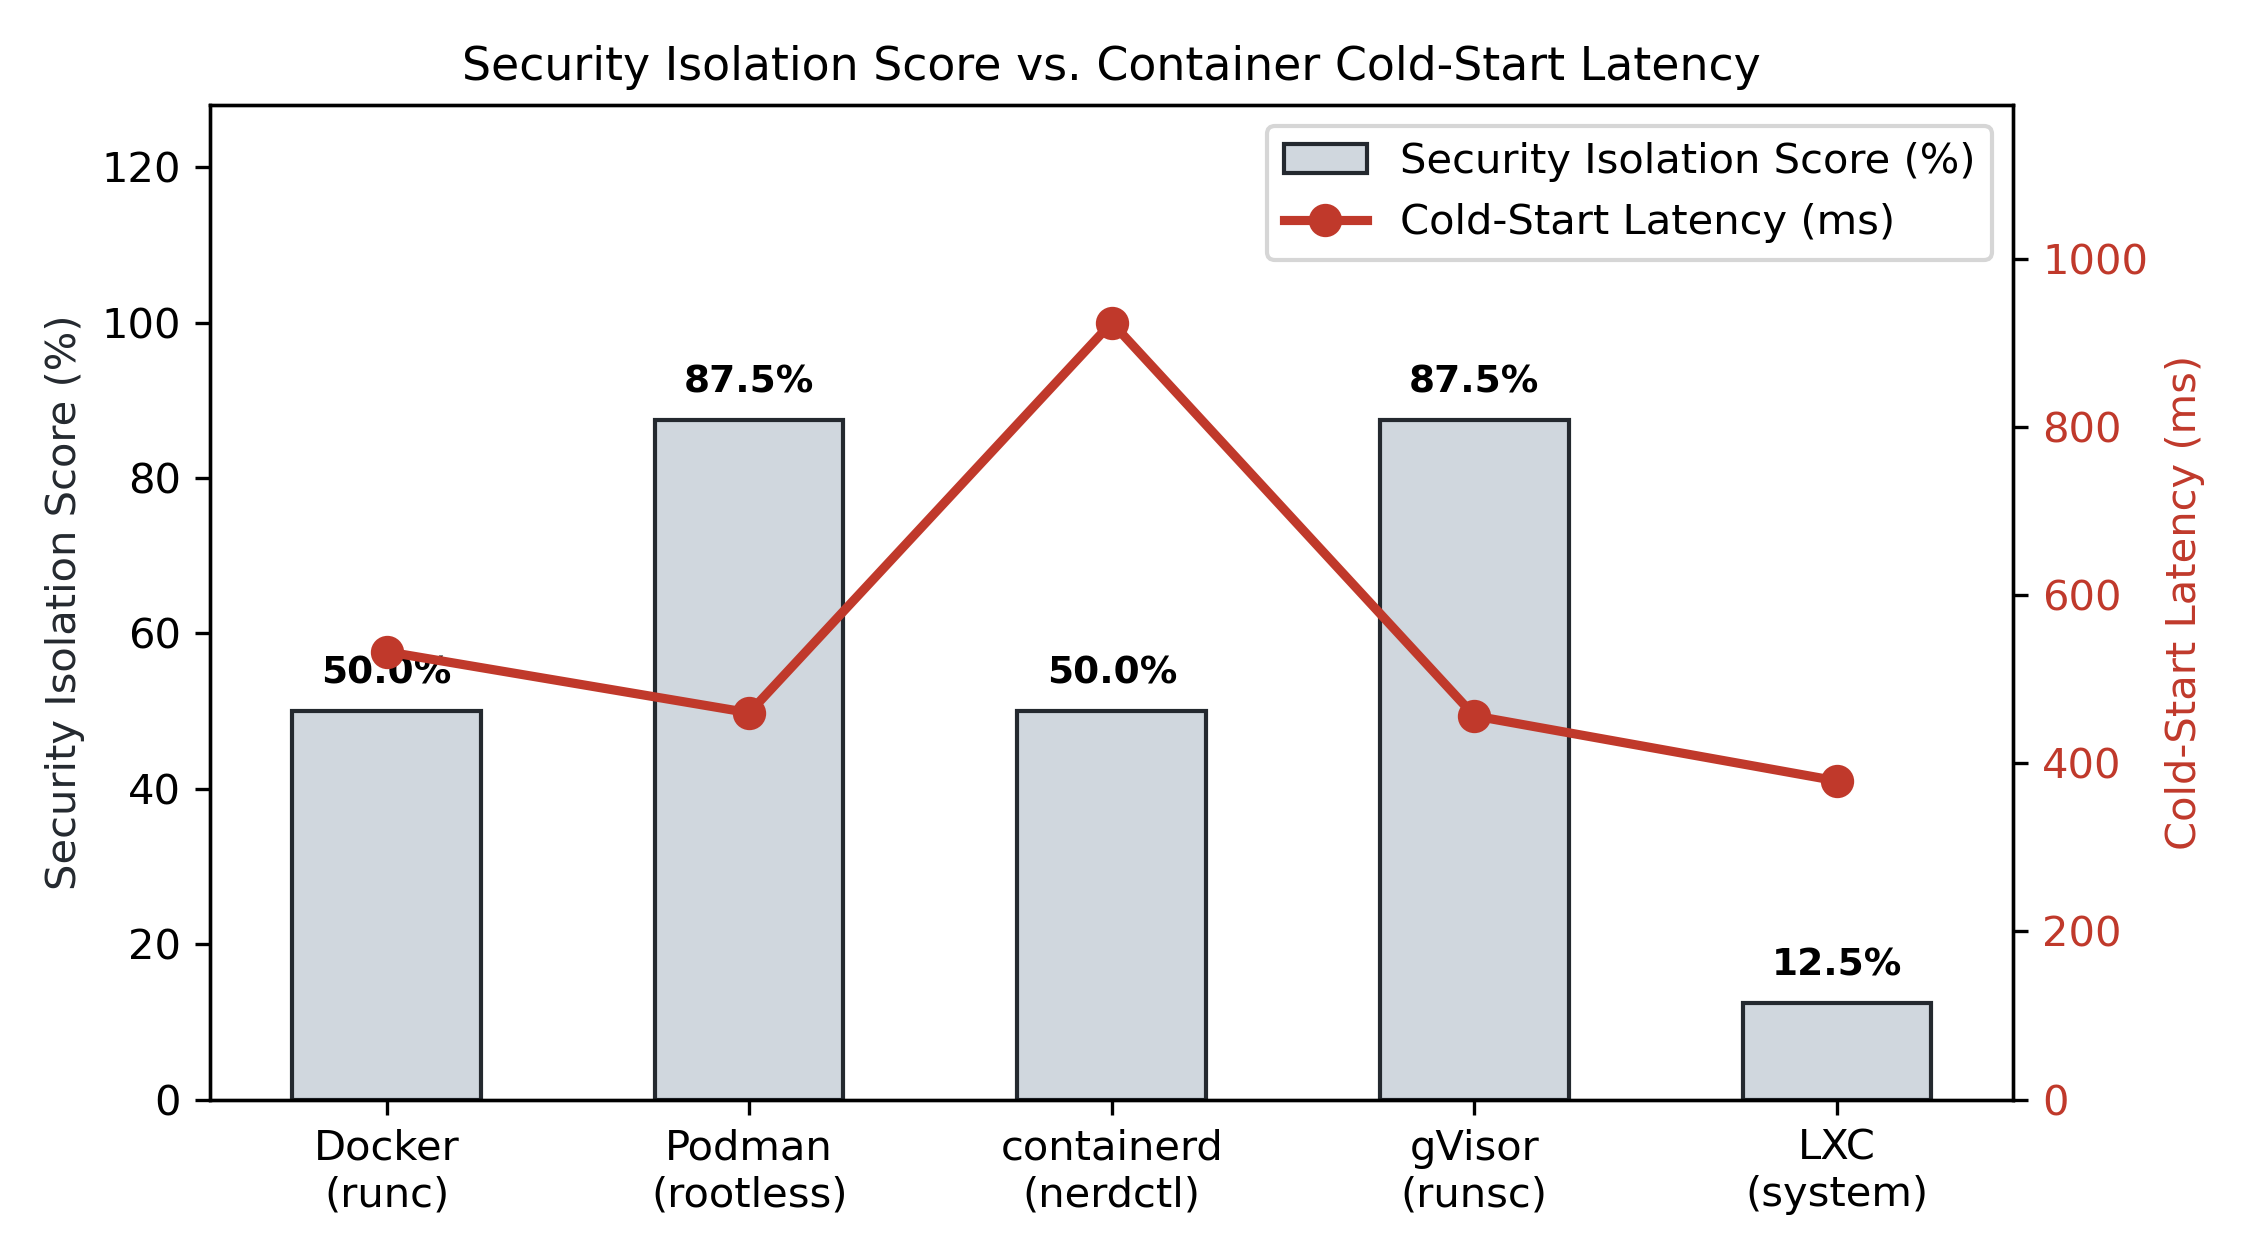
\includegraphics[width=\linewidth]{fig1_isolation_vs_startup.png}
\caption{Module 1 basic security score vs.\ cold-start latency across all five runtimes.}
\label{fig:fig1}
\end{figure}

\begin{figure}[t]
\centering
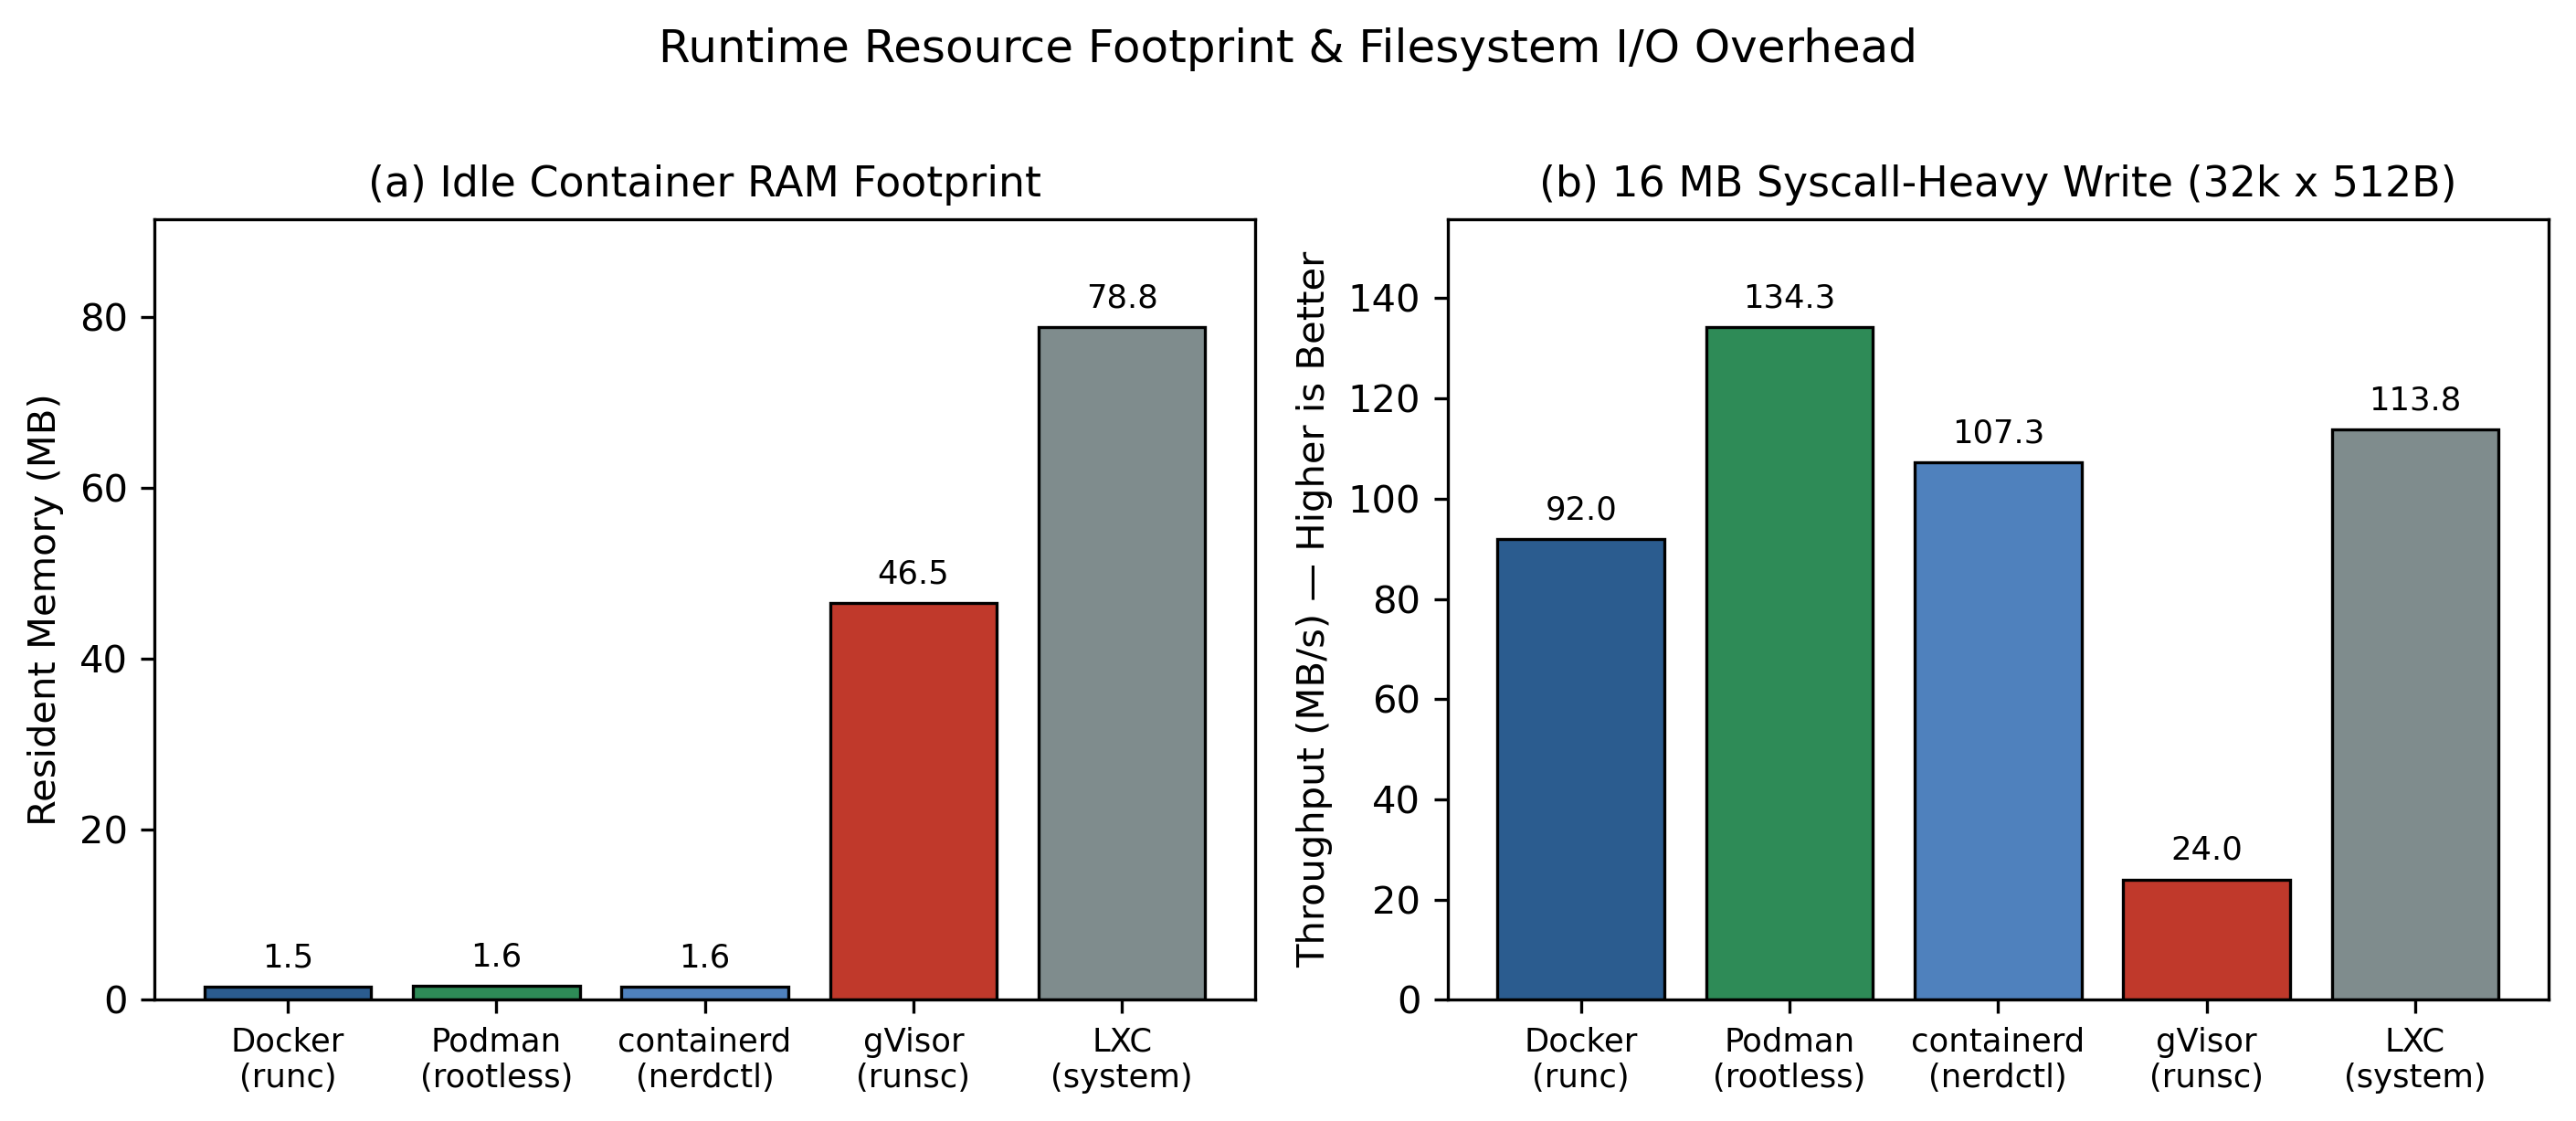
\includegraphics[width=\linewidth]{fig2_resource_io_overhead.png}
\caption{Idle container RAM usage and 16~MB small-block disk write speed.}
\label{fig:fig2}
\end{figure}

\begin{figure}[t]
\centering
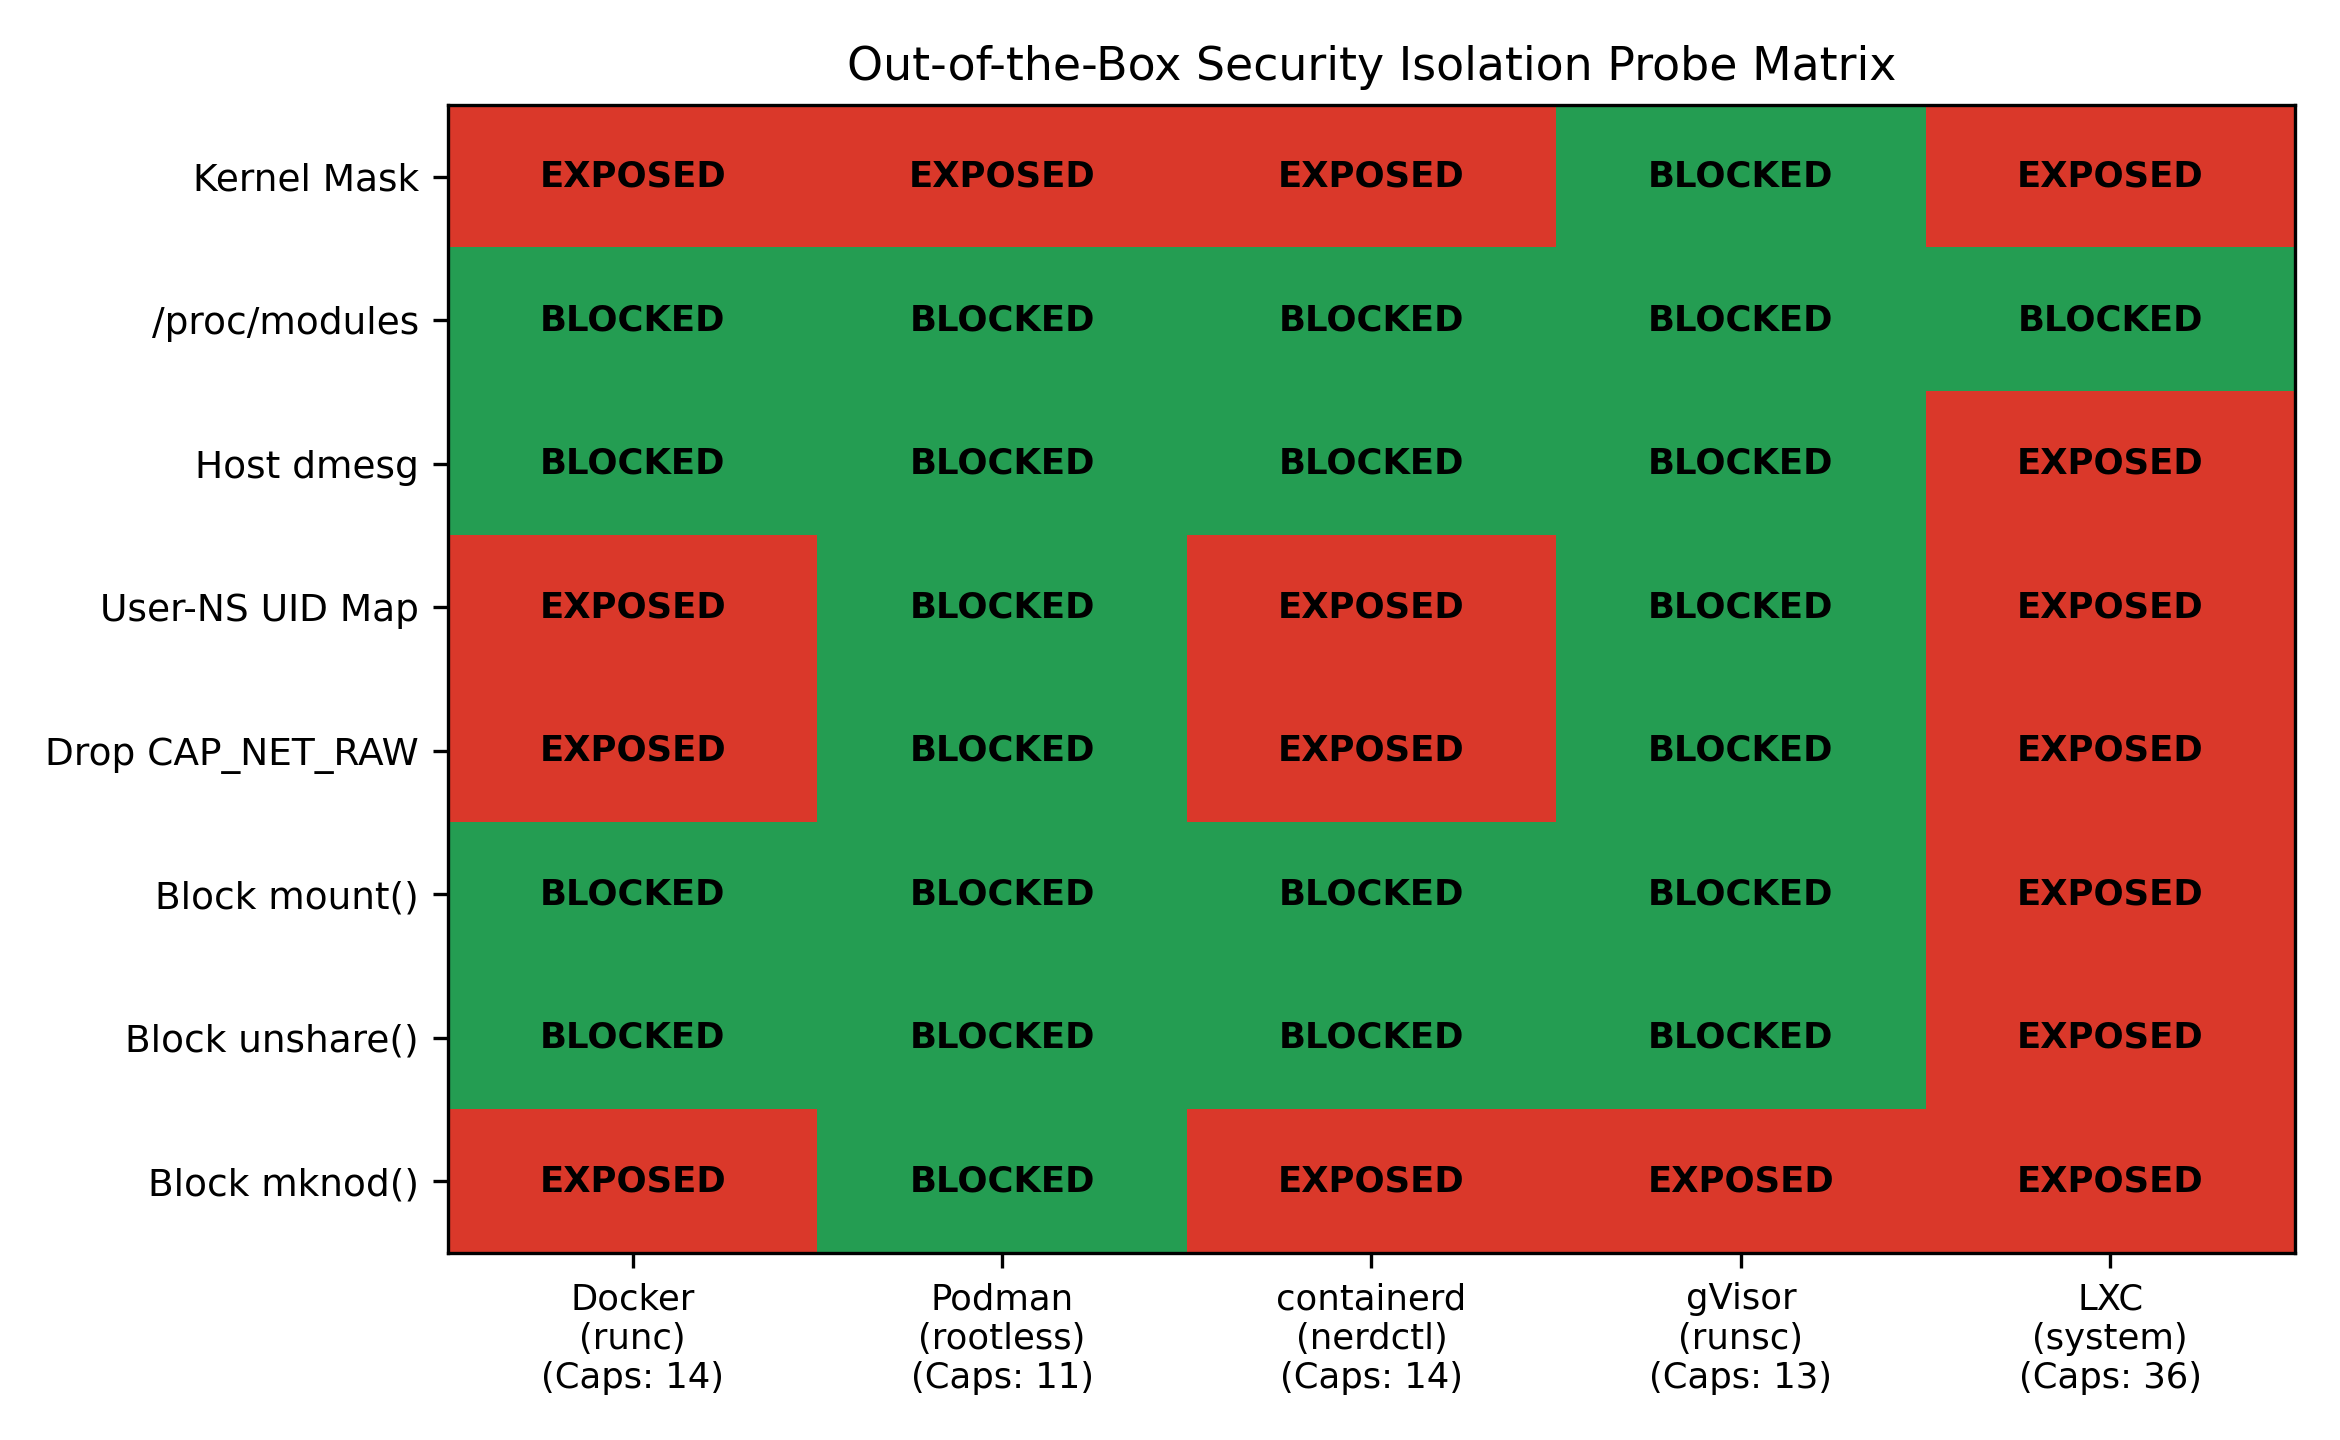
\includegraphics[width=\linewidth]{fig3_security_probe_heatmap.png}
\caption{Module 1 8-point security check matrix and default Linux capability counts.}
\label{fig:fig3}
\end{figure}

\begin{figure}[t]
\centering
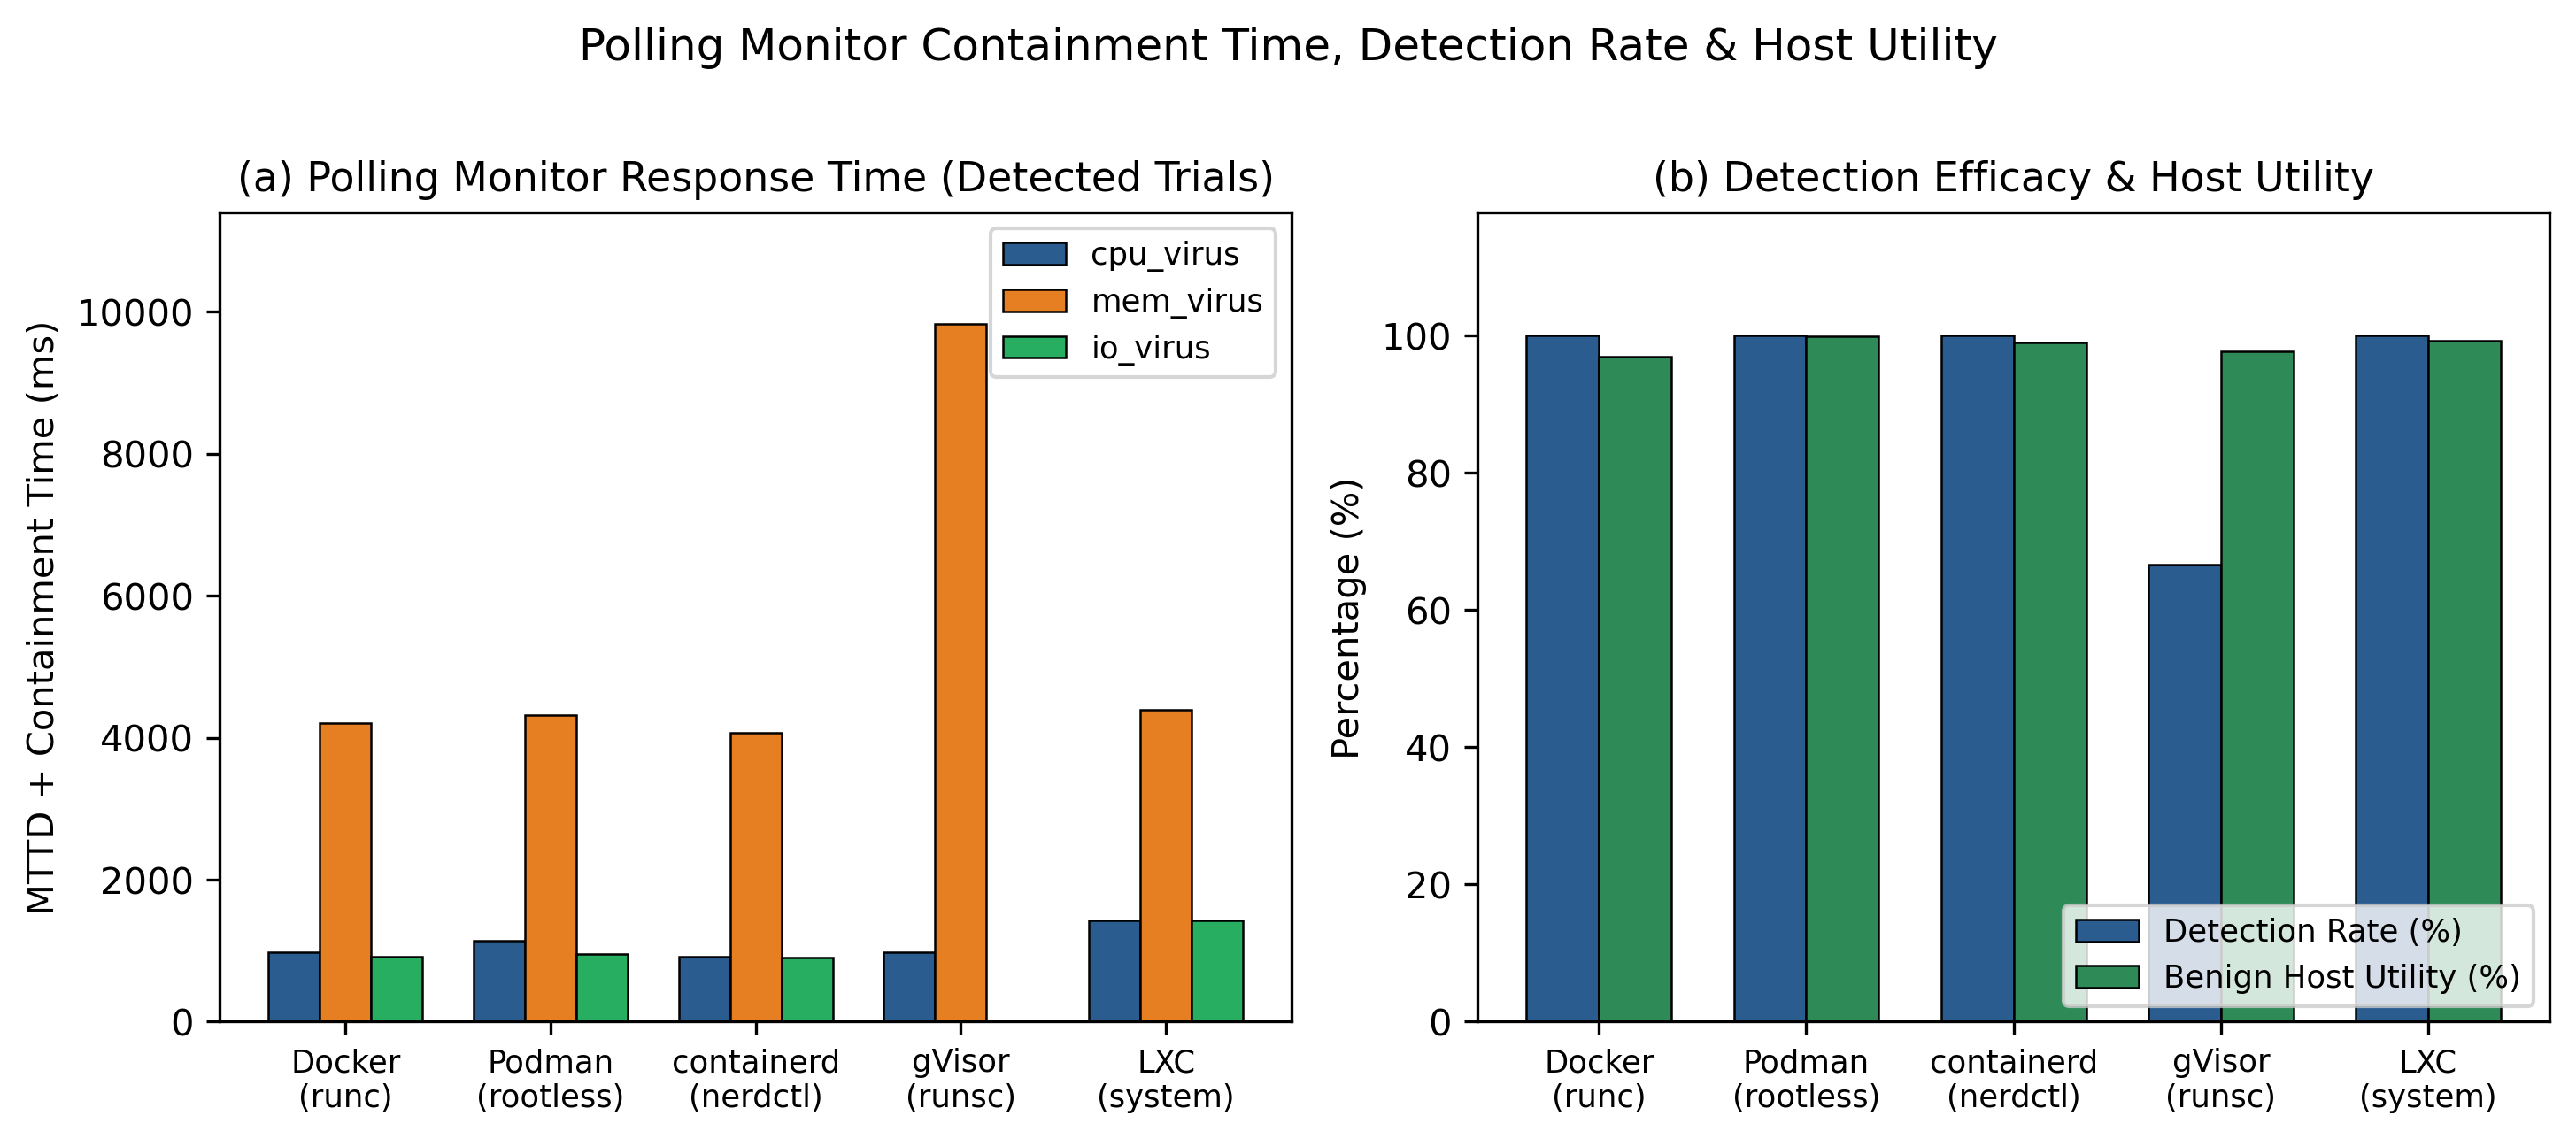
\includegraphics[width=\linewidth]{fig4_blueteam_and_host_utility.png}
\caption{Module 1 polling monitor response time, detection rate, and host utility.}
\label{fig:fig4}
\end{figure}

\subsection{Module 2: System Call and Network Benchmarks}
Tables~\ref{tab:m2_syscall} and~\ref{tab:m2_net} present the 5-trial system call and network measurements (visualized in Figs.~\ref{fig:fig5} and~\ref{fig:fig6}).

\begin{table*}[t]
\centering
\caption{Module 2 System Call Latency (Mean ns/op and Ratio vs.\ Bare Host, 5 Trials)}
\label{tab:m2_syscall}
\begin{tabular}{lccccc}
\toprule
\textbf{Runtime} & \textbf{\texttt{getpid()}} & \textbf{\texttt{open()+close()}} & \textbf{\texttt{pipe()} R/W} & \textbf{\texttt{mmap+fault+munmap}} & \textbf{\texttt{fork()+waitpid()}} \\
\midrule
Bare Host (control)           & 815.6 (1.00$\times$) & 2,815.1 (1.00$\times$) & 1,957.2 (1.00$\times$) & 11,013.4 (1.00$\times$) & 379,273.1 (1.00$\times$) \\
Docker (\texttt{runc})        & 1,130.3 (1.39$\times$) & 3,832.4 (1.36$\times$) & 2,132.1 (1.09$\times$) & 11,110.3 (1.01$\times$) & 294,451.9 (0.78$\times$) \\
Podman (rootless)             & 845.7 (1.04$\times$) & 3,042.8 (1.08$\times$) & 2,031.0 (1.04$\times$) & 11,717.4 (1.06$\times$) & 364,395.9 (0.96$\times$) \\
containerd (\texttt{nerdctl}) & 994.1 (1.22$\times$) & 3,684.7 (1.31$\times$) & 2,048.0 (1.05$\times$) & 10,949.9 (0.99$\times$) & 351,985.9 (0.93$\times$) \\
gVisor (\texttt{runsc})       & \textbf{15,236.6 (18.68$\times$)} & \textbf{9,136.8 (3.25$\times$)} & \textbf{9,309.5 (4.76$\times$)} & \textbf{337,946.0 (30.68$\times$)} & \textbf{3,767,931.4 (9.93$\times$)} \\
LXC (system)                  & 854.4 (1.05$\times$) & 3,354.5 (1.19$\times$) & 2,062.5 (1.05$\times$) & 11,240.0 (1.02$\times$) & 373,245.1 (0.98$\times$) \\
\bottomrule
\end{tabular}
\end{table*}

\begin{table}[t]
\centering
\caption{Module 2 Container-to-Host Network Speed and \texttt{SOCK\_RAW} Check (Mean $\pm$ Std, 5 Trials)}
\label{tab:m2_net}
\begin{tabular}{lccc}
\toprule
\textbf{Runtime} & \textbf{TCP RTT ($\mu$s)} & \textbf{Throughput (MB/s)} & \textbf{\texttt{SOCK\_RAW}} \\
\midrule
Bare Host  & 120.79 $\pm$ 3.51  & 1769.93 $\pm$ 180.92 & EXPOSED \\
Docker     & \textbf{58.91 $\pm$ 21.71}  & \textbf{1968.68 $\pm$ 821.81} & EXPOSED \\
Podman     & 264.78 $\pm$ 5.37  & 641.69 $\pm$ 729.41  & \textbf{BLOCKED} \\
containerd & \textbf{55.77 $\pm$ 22.59}  & 1796.03 $\pm$ 482.21 & EXPOSED \\
gVisor     & 289.48 $\pm$ 29.58 & 573.38 $\pm$ 108.75  & \textbf{BLOCKED} \\
LXC        & 119.33 $\pm$ 16.19 & 1840.48 $\pm$ 176.29 & EXPOSED \\
\bottomrule
\end{tabular}
\end{table}

On system calls, all four shared-kernel runtimes performed close to the bare host across every tested operation, showing that namespaces and rootless user mapping add very little syscall delay. In contrast, gVisor was significantly slower across the board---from more than 3$\times$ slower on \texttt{open()+close()} up to over 30$\times$ slower on memory page mapping and faulting---directly explaining its low disk I/O result in Module~1.

Networking showed a clear split between speed and packet safety. Docker, containerd, and LXC delivered fast TCP transfers and low round-trip times, but all three allowed containers to create raw ICMP sockets. Rootless Podman and gVisor were the only runtimes that blocked \texttt{SOCK\_RAW}, yet both showed noticeably higher TCP latency and lower average throughput because their traffic passes through user-space networking layers. Podman also showed wide trial-to-trial variation on bulk TCP transfers, ranging from 50.64 to 1,497.86~MB/s across its five trials.

\begin{figure}[t]
\centering
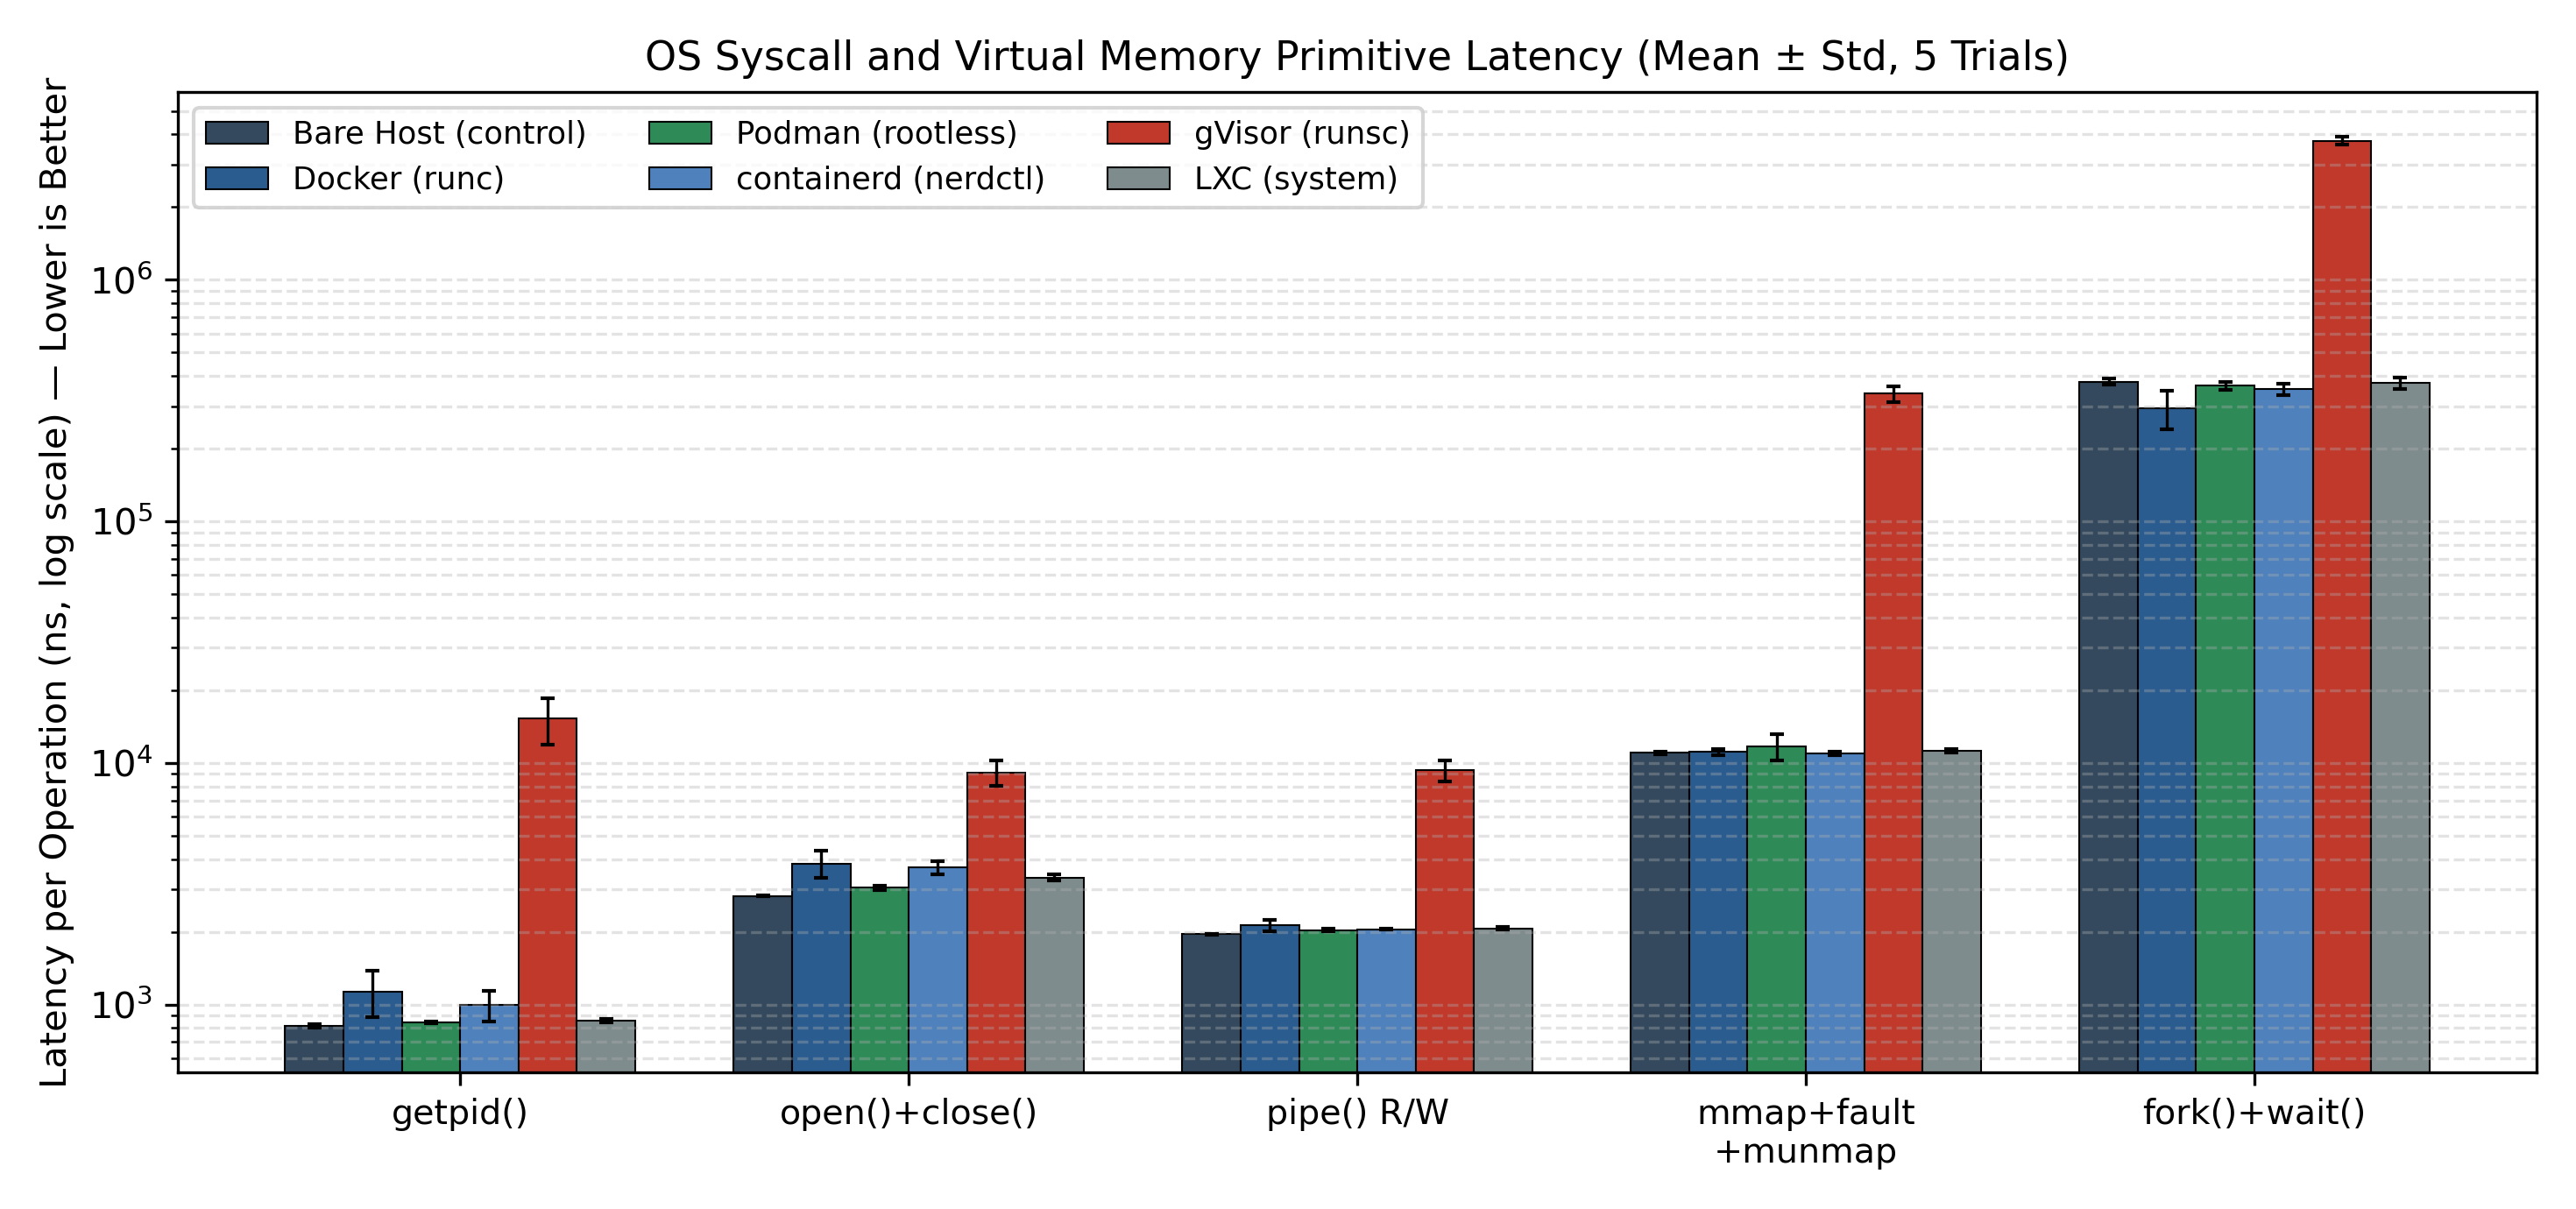
\includegraphics[width=\linewidth]{fig5_syscall_microbench.png}
\caption{System call latency (log scale) across five Linux operations (5 trials).}
\label{fig:fig5}
\end{figure}

\begin{figure}[t]
\centering
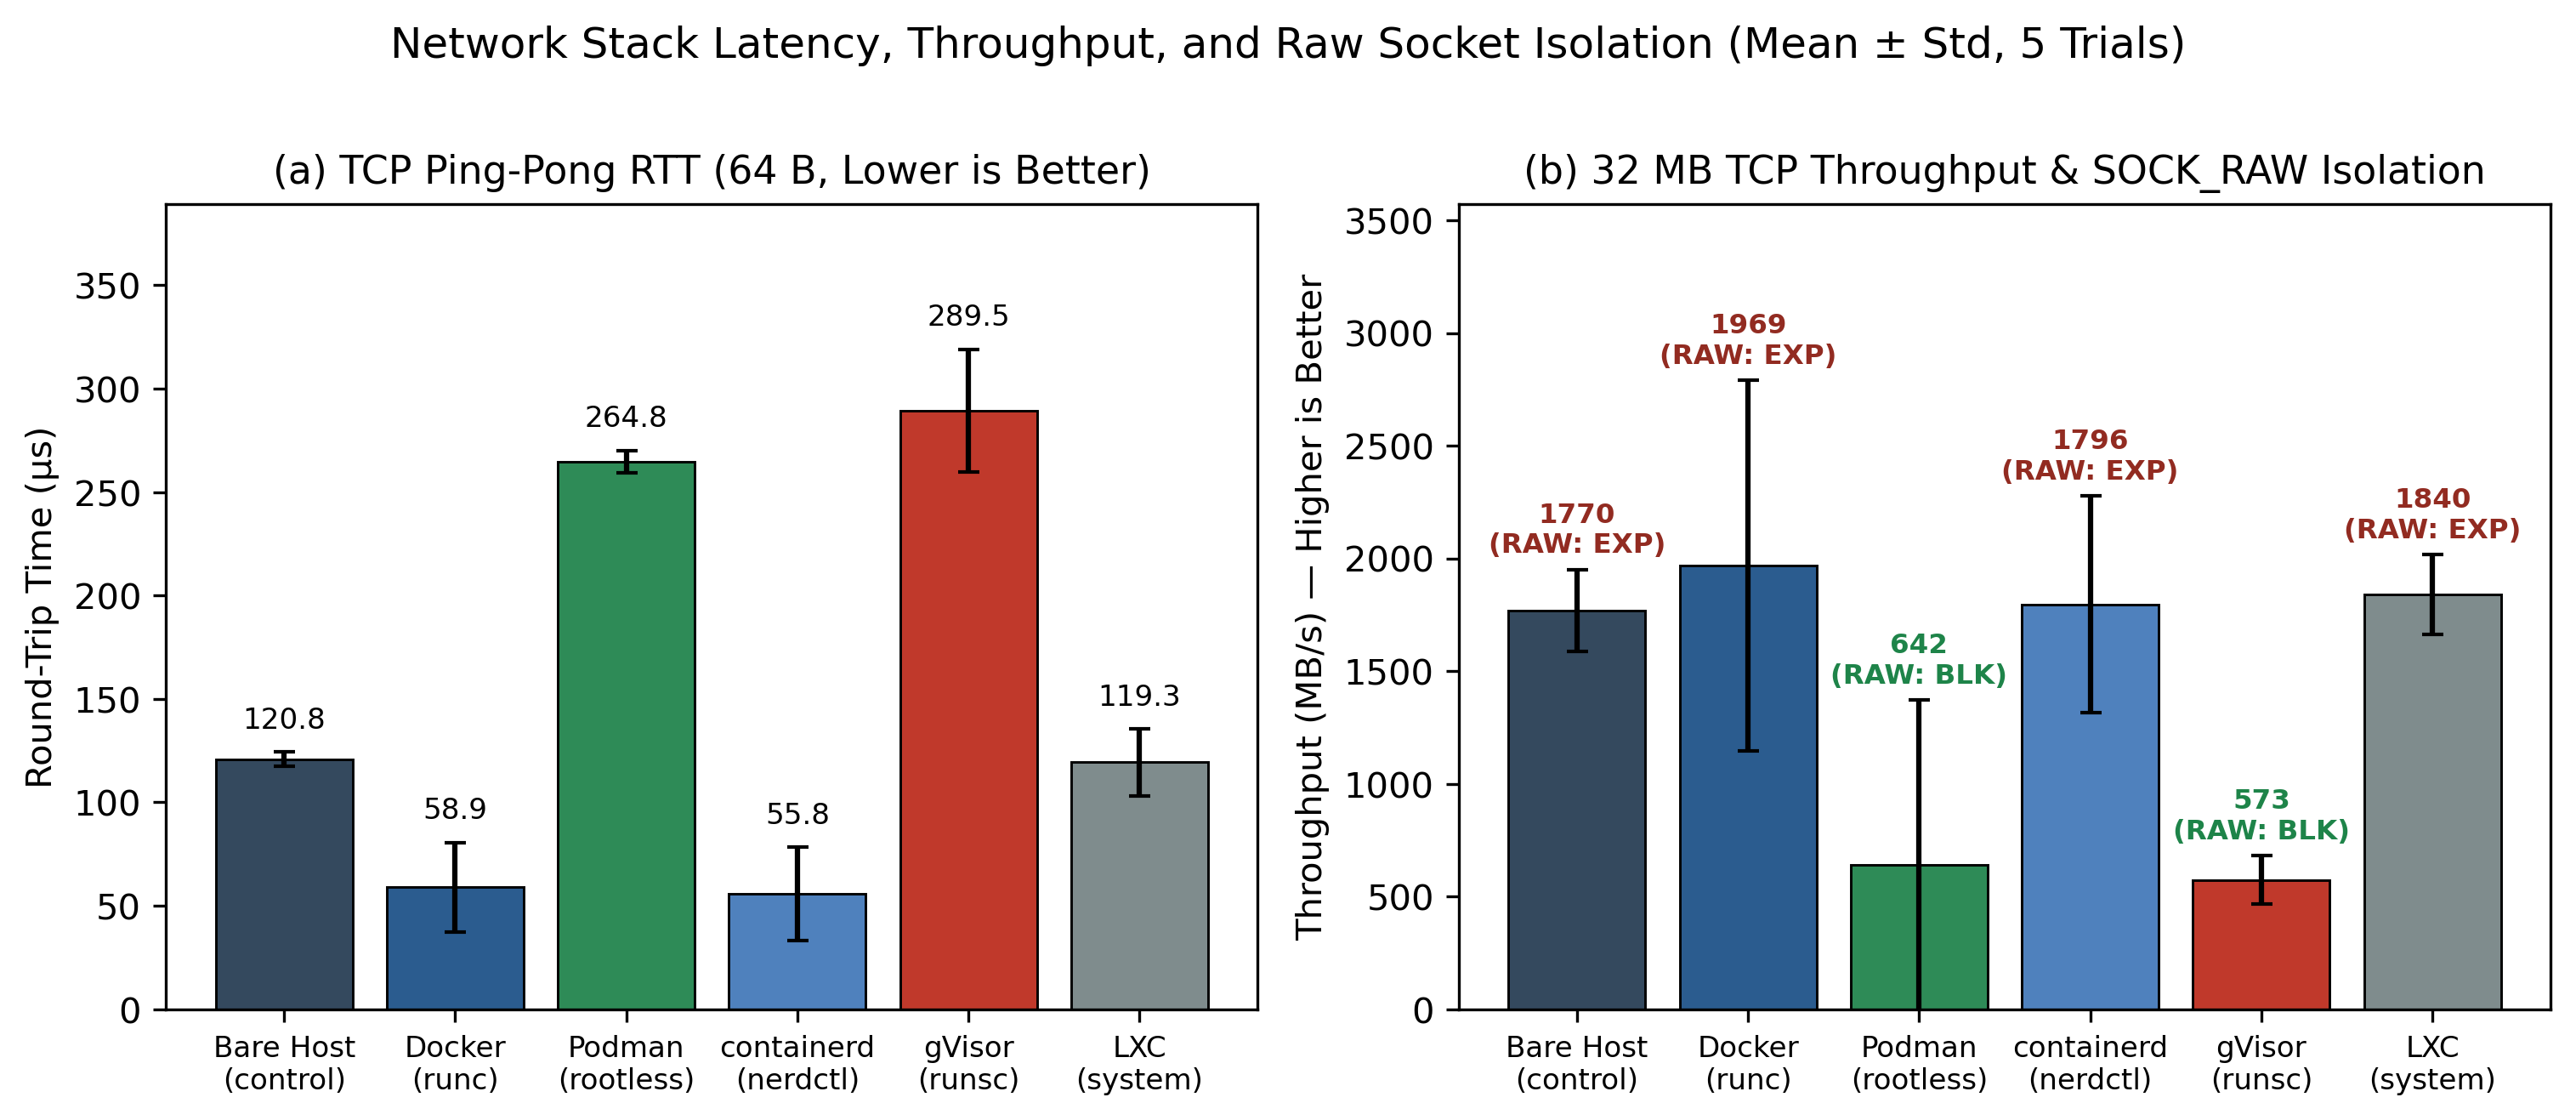
\includegraphics[width=\linewidth]{fig6_network_overhead.png}
\caption{Container-to-host TCP round-trip time, 32~MB throughput, and \texttt{SOCK\_RAW} results (5 trials).}
\label{fig:fig6}
\end{figure}

\subsection{Module 3: Active Security Audit, Fork Bomb, and CPU Starvation}
Table~\ref{tab:m3_summary} and Figs.~\ref{fig:fig7}--\ref{fig:fig8} show the results of the expanded 15-check audit and stress containment tests.

\begin{table*}[t]
\centering
\caption{Module 3 Active Security Audit (15 Checks), Fork-Bomb Containment, and 8-Thread CPU Starvation (Mean $\pm$ Std, 3 Trials)}
\label{tab:m3_summary}
\begin{tabular}{lccccccc}
\toprule
\textbf{Runtime} & \textbf{15-Check} & \textbf{\texttt{P10} \texttt{bpf()}} & \textbf{\texttt{P15} Secret} & \textbf{Fork Bomb} & \textbf{Fork Bomb} & \textbf{Host Util. (\%)} & \textbf{Host Util. (\%)} \\
 & \textbf{Blocked (\%)} & \textbf{Syscall} & \textbf{Mount} & \textbf{Default} & \textbf{Cap (64 PIDs)} & \textbf{Unconstrained} & \textbf{Capped (1 CPU)} \\
\midrule
Docker (\texttt{runc})        & 8/15 (53.3\%)  & BLOCKED & EXPOSED & 500/500 & 63 (\texttt{EAGAIN}) & 56.95 $\pm$ 1.52 & 83.34 $\pm$ 0.73 \\
Podman (rootless)             & \textbf{11/15 (73.3\%)} & BLOCKED & \textbf{BLOCKED} & 500/500 & 63 (\texttt{EAGAIN}) & 56.39 $\pm$ 0.56 & 82.59 $\pm$ 0.27 \\
containerd (\texttt{nerdctl}) & 8/15 (53.3\%)  & BLOCKED & EXPOSED & 500/500 & 63 (\texttt{EAGAIN}) & 58.32 $\pm$ 0.32 & 80.51 $\pm$ 3.78 \\
gVisor (\texttt{runsc})       & 10/15 (66.7\%) & BLOCKED & EXPOSED & 500/500 & Exit 2 (no output)   & 55.52 $\pm$ 2.29 & \textbf{85.00 $\pm$ 0.53} \\
LXC (system)                  & 2/15 (13.3\%)  & EXPOSED & EXPOSED & 500/500 & 47 (\texttt{EAGAIN}) & 55.29 $\pm$ 2.82 & 83.84 $\pm$ 1.93 \\
\bottomrule
\end{tabular}
\end{table*}

Expanding to 15 checks broke the Module~1 tie between Podman and gVisor. Rootless Podman finished first because it was the only runtime that blocked reading the bind-mounted host \texttt{root:root} secret file (\texttt{P15}): since container root maps to an unprivileged host user, Linux denied file access. Under rootful Docker, containerd, gVisor, and LXC, container root read the file. gVisor still finished second overall by hiding the real kernel version (\texttt{4.19.0-gvisor}) and blocking \texttt{keyctl()}, though it left \texttt{/proc/sysrq-trigger} writable (while keeping \texttt{/sys} read-only). Docker and containerd tied identically, while default LXC scored lowest and even allowed creating a real kernel eBPF map (\texttt{P10}) as well as \texttt{setns()}, \texttt{mount()}, and \texttt{unshare()}.

In the stress tests, no runtime stopped the 500-process fork bomb or prevented 8-thread CPU starvation under default settings---host throughput dropped nearly in half across all five runtimes. Adding a 64-PID cgroup limit stopped the fork bomb cleanly with an \texttt{EAGAIN} error on Docker, Podman, containerd, and LXC (LXC allowed fewer child processes because background tasks inside the container used part of the 64-PID quota). Under gVisor, the 64-PID cap allowed a small 10-process check to pass (\texttt{exit=0}) but terminated the 500-process run with exit code~2 and no output. Adding a 1-CPU cgroup limit restored host CPU throughput above 80\% on every runtime.

\begin{figure}[t]
\centering
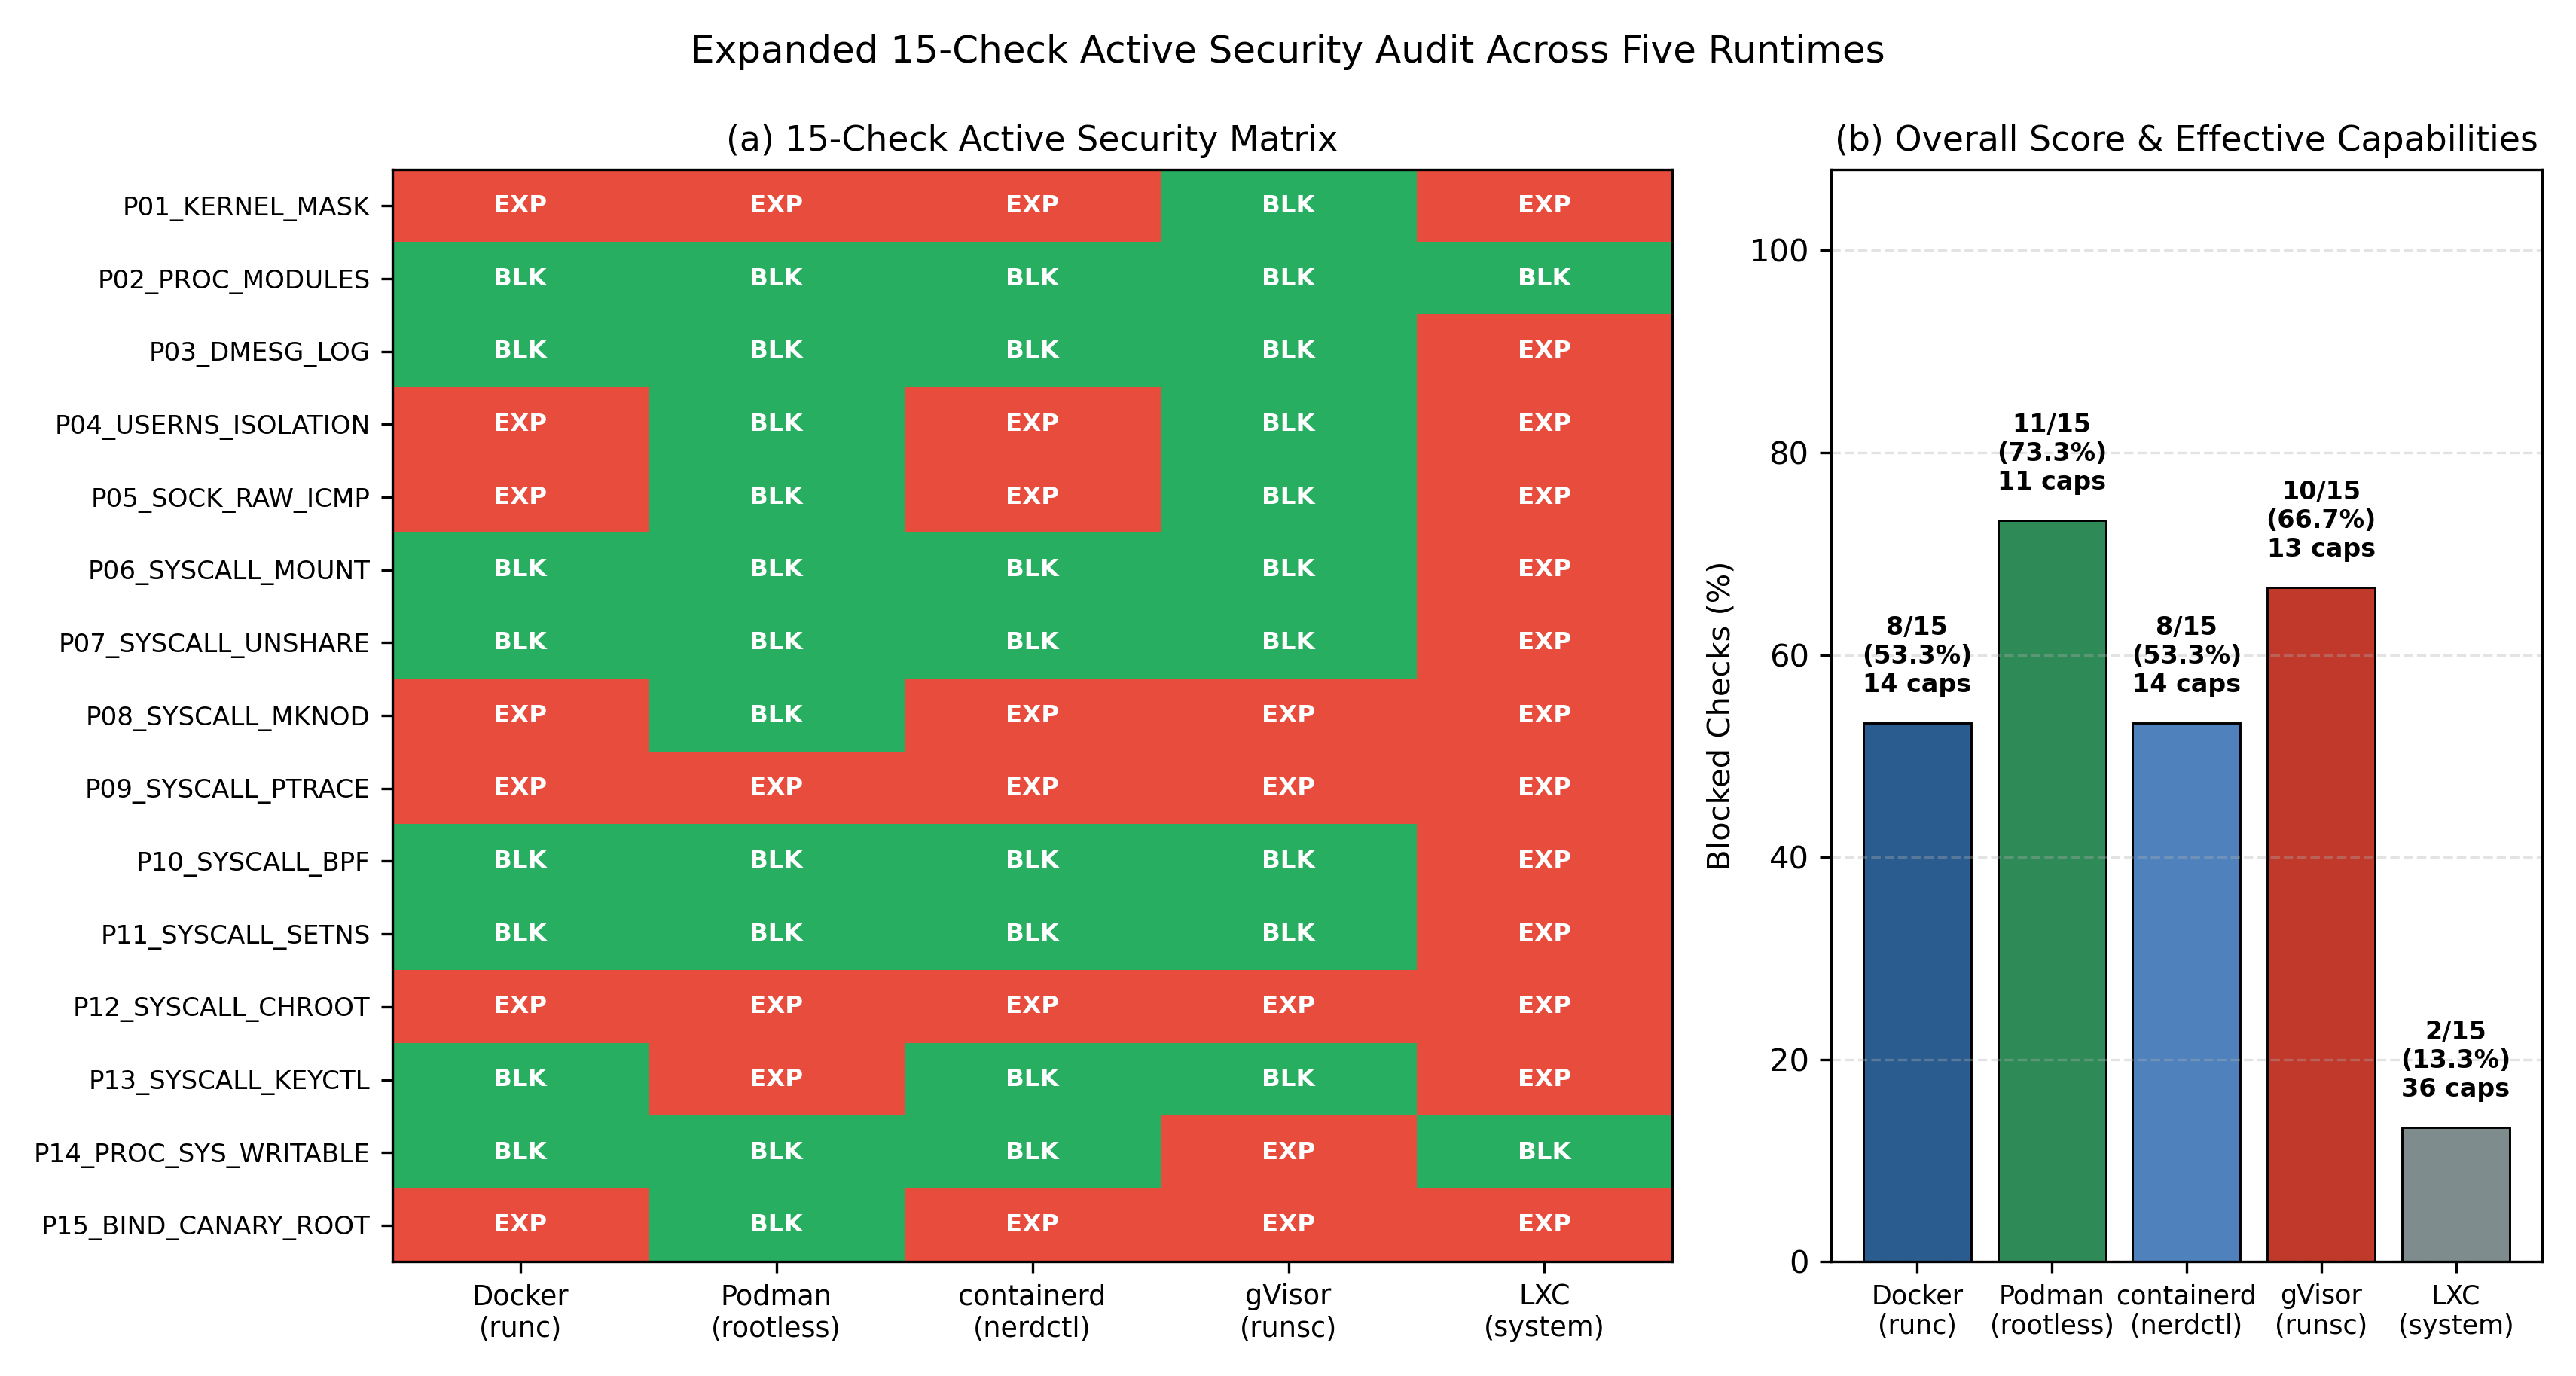
\includegraphics[width=\linewidth]{fig7_escape_matrix_v2.png}
\caption{15-check active security matrix and effective capability counts across all five runtimes.}
\label{fig:fig7}
\end{figure}

\begin{figure}[t]
\centering
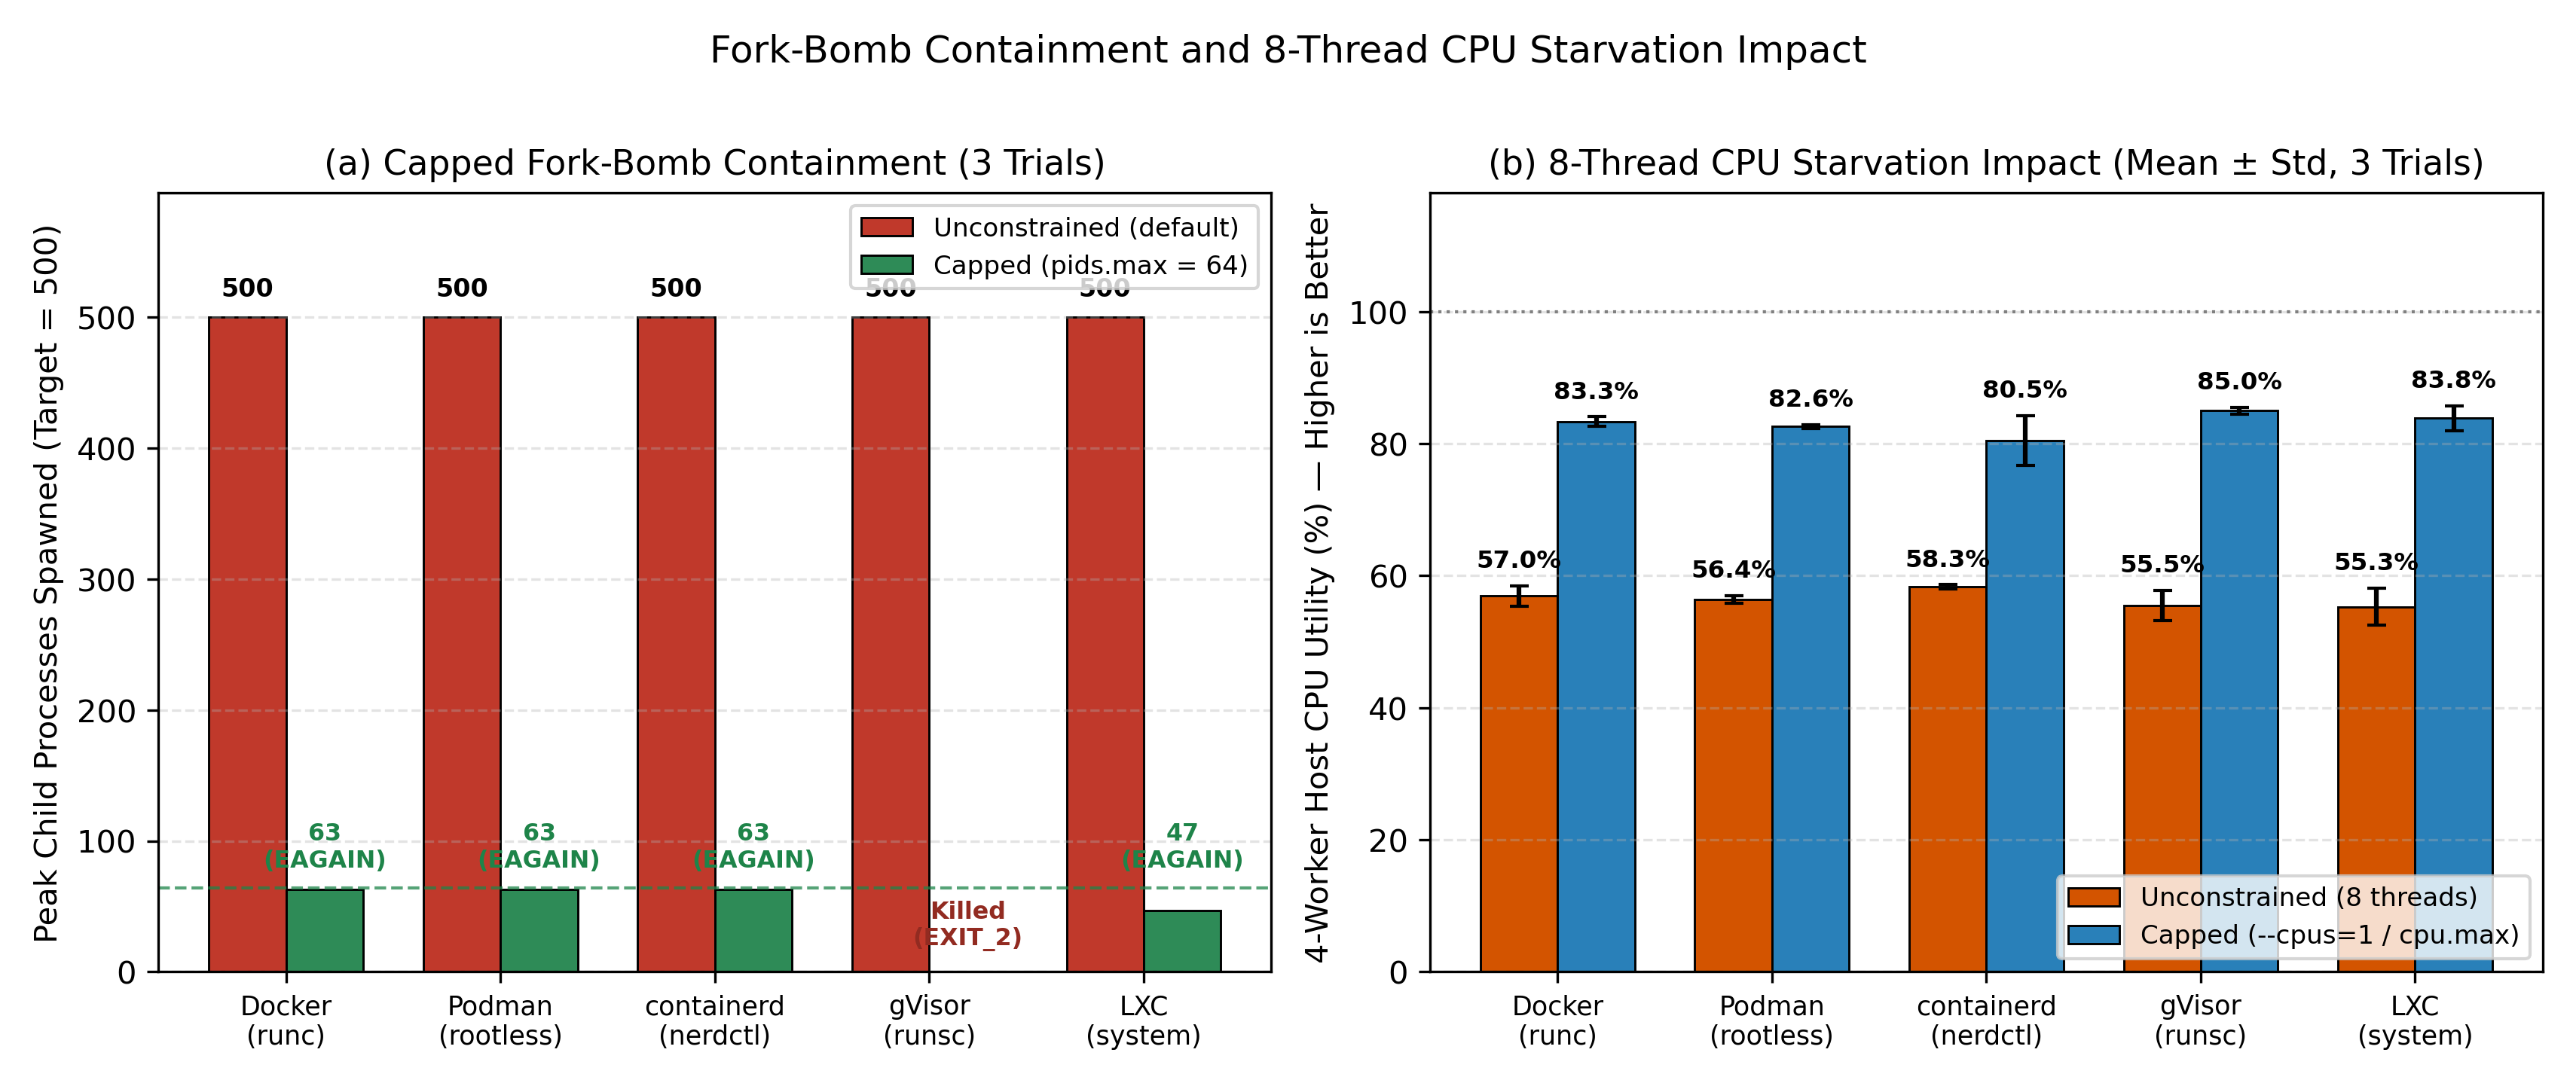
\includegraphics[width=\linewidth]{fig8_forkbomb_and_starvation.png}
\caption{Fork-bomb containment (default vs.\ 64-PID cap) and 8-thread CPU starvation impact (default vs.\ 1-CPU cap).}
\label{fig:fig8}
\end{figure}

\subsection{Module 4: Kernel eBPF Monitor and Weighted Comparison}
Table~\ref{tab:m4_ebpf} and Fig.~\ref{fig:fig9} compare the 135 polling trials from Module~1 against the 135 kernel eBPF trials in Module~4, while Fig.~\ref{fig:fig10} shows how stealth Levels~1--3 affected polling detection times.

\begin{table*}[t]
\centering
\caption{Module 4 Host Monitor Comparison: User-Space Polling (135 Trials) vs.\ Kernel eBPF (135 Trials)}
\label{tab:m4_ebpf}
\begin{tabular}{lccccccc}
\toprule
\textbf{Runtime} & \textbf{Polling} & \textbf{Polling Resp.} & \textbf{eBPF} & \textbf{eBPF Kernel} & \textbf{eBPF Resp.} & \textbf{Response} & \textbf{Level 3 Spoof} \\
 & \textbf{Det. (\%)} & \textbf{(ms)} & \textbf{Det. (\%)} & \textbf{MTTD (ms)} & \textbf{(ms)} & \textbf{Speedup} & \textbf{Caught (\%)} \\
\midrule
Docker (\texttt{runc})        & 100.0 & 2,029.3 & \textbf{100.0} & 4.91 & 548.6 & 3.70$\times$ & \textbf{100.0} \\
Podman (rootless)             & 100.0 & 2,136.8 & \textbf{100.0} & 4.12 & \textbf{544.6} & \textbf{3.92$\times$} & \textbf{100.0} \\
containerd (\texttt{nerdctl}) & 100.0 & \textbf{1,965.4} & \textbf{100.0} & 5.73 & 956.6 & 2.05$\times$ & \textbf{100.0} \\
gVisor (\texttt{runsc})       & 66.7  & 5,399.6 & \textbf{0.0}   & ---  & ---   & ---          & \textbf{0.0}   \\
LXC (system)                  & 100.0 & 2,412.9 & \textbf{100.0} & \textbf{3.08} & 776.6 & 3.11$\times$ & \textbf{100.0} \\
\bottomrule
\end{tabular}
\end{table*}

On the four shared-kernel runtimes (Docker, Podman, containerd, and LXC), kernel eBPF caught every attack within a few milliseconds of startup, cut total launch-to-kill time by 2$\times$ to nearly 4$\times$, and flagged every Level~3 process-renaming attempt. On gVisor, however, host kernel eBPF caught zero attacks and saw none of the renaming attempts because container system calls were intercepted by Sentry and never triggered host kernel tracepoints.

Fig.~\ref{fig:fig10} illustrates why polling struggles against stealthy behavior. When \texttt{mem\_virus} slowed down its memory allocation in Levels~2 and~3, polling detection time jumped from roughly 0.2--0.7~s up to 5.4--5.7~s on native runtimes and roughly 14~s on gVisor. Similarly, slowed \texttt{io\_virus} runs delayed polling detection from under 0.3~s to nearly 1~s on native runtimes (while remaining undetected on gVisor). Under kernel eBPF on shared-kernel runtimes, detection time stayed flat between 3.01 and 7.38~ms regardless of stealth level.

Table~\ref{tab:m4_matrix} and Fig.~\ref{fig:fig11} combine all four modules into normalized 0--100 scores across three example weighting profiles: \textit{General / Monitored} (30\% Security, 20\% Syscall/Disk, 15\% Network, 15\% Efficiency, 20\% Visibility), \textit{High-Throughput} (15\% Security, 25\% Syscall/Disk, 35\% Network, 15\% Efficiency, 10\% Visibility), and \textit{Security-First} (55\% Security, 15\% Syscall/Disk, 5\% Network, 10\% Efficiency, 15\% Visibility).

\begin{table*}[t]
\centering
\caption{Normalized Empirical Scores (0--100) and Example Weighted Deployment Profile Rankings}
\label{tab:m4_matrix}
\begin{tabular}{lcccccccc}
\toprule
\textbf{Runtime} & \textbf{Security} & \textbf{Syscall \&} & \textbf{Network} & \textbf{Startup \&} & \textbf{Host} & \textbf{General /} & \textbf{High-} & \textbf{Security-} \\
 & \textbf{(15-Check)} & \textbf{Disk I/O} & \textbf{(TCP)} & \textbf{RAM Eff.} & \textbf{Visibility} & \textbf{Monitored} & \textbf{Throughput} & \textbf{First} \\
\midrule
Docker (\texttt{runc})        & 53.3 & 81.2  & \textbf{97.3} & 85.6 & \textbf{100.0} & \textbf{79.7} & \textbf{85.2} & 69.9 \\
Podman (rootless)             & \textbf{73.3} & \textbf{100.0} & 26.8 & \textbf{88.1} & \textbf{100.0} & 79.2 & 68.6 & \textbf{80.5} \\
containerd (\texttt{nerdctl}) & 53.3 & 87.4  & 95.6 & 67.4 & \textbf{100.0} & 77.9 & 83.4 & 68.9 \\
gVisor (\texttt{runsc})       & 66.7 & 14.2  & 24.2 & 43.1 & 33.4  & 39.6 & 31.8 & 49.3 \\
LXC (system)                  & 13.3 & 91.4  & 70.1 & 51.0 & \textbf{100.0} & 60.4 & 67.0 & 44.6 \\
\bottomrule
\end{tabular}
\end{table*}

\begin{figure}[t]
\centering
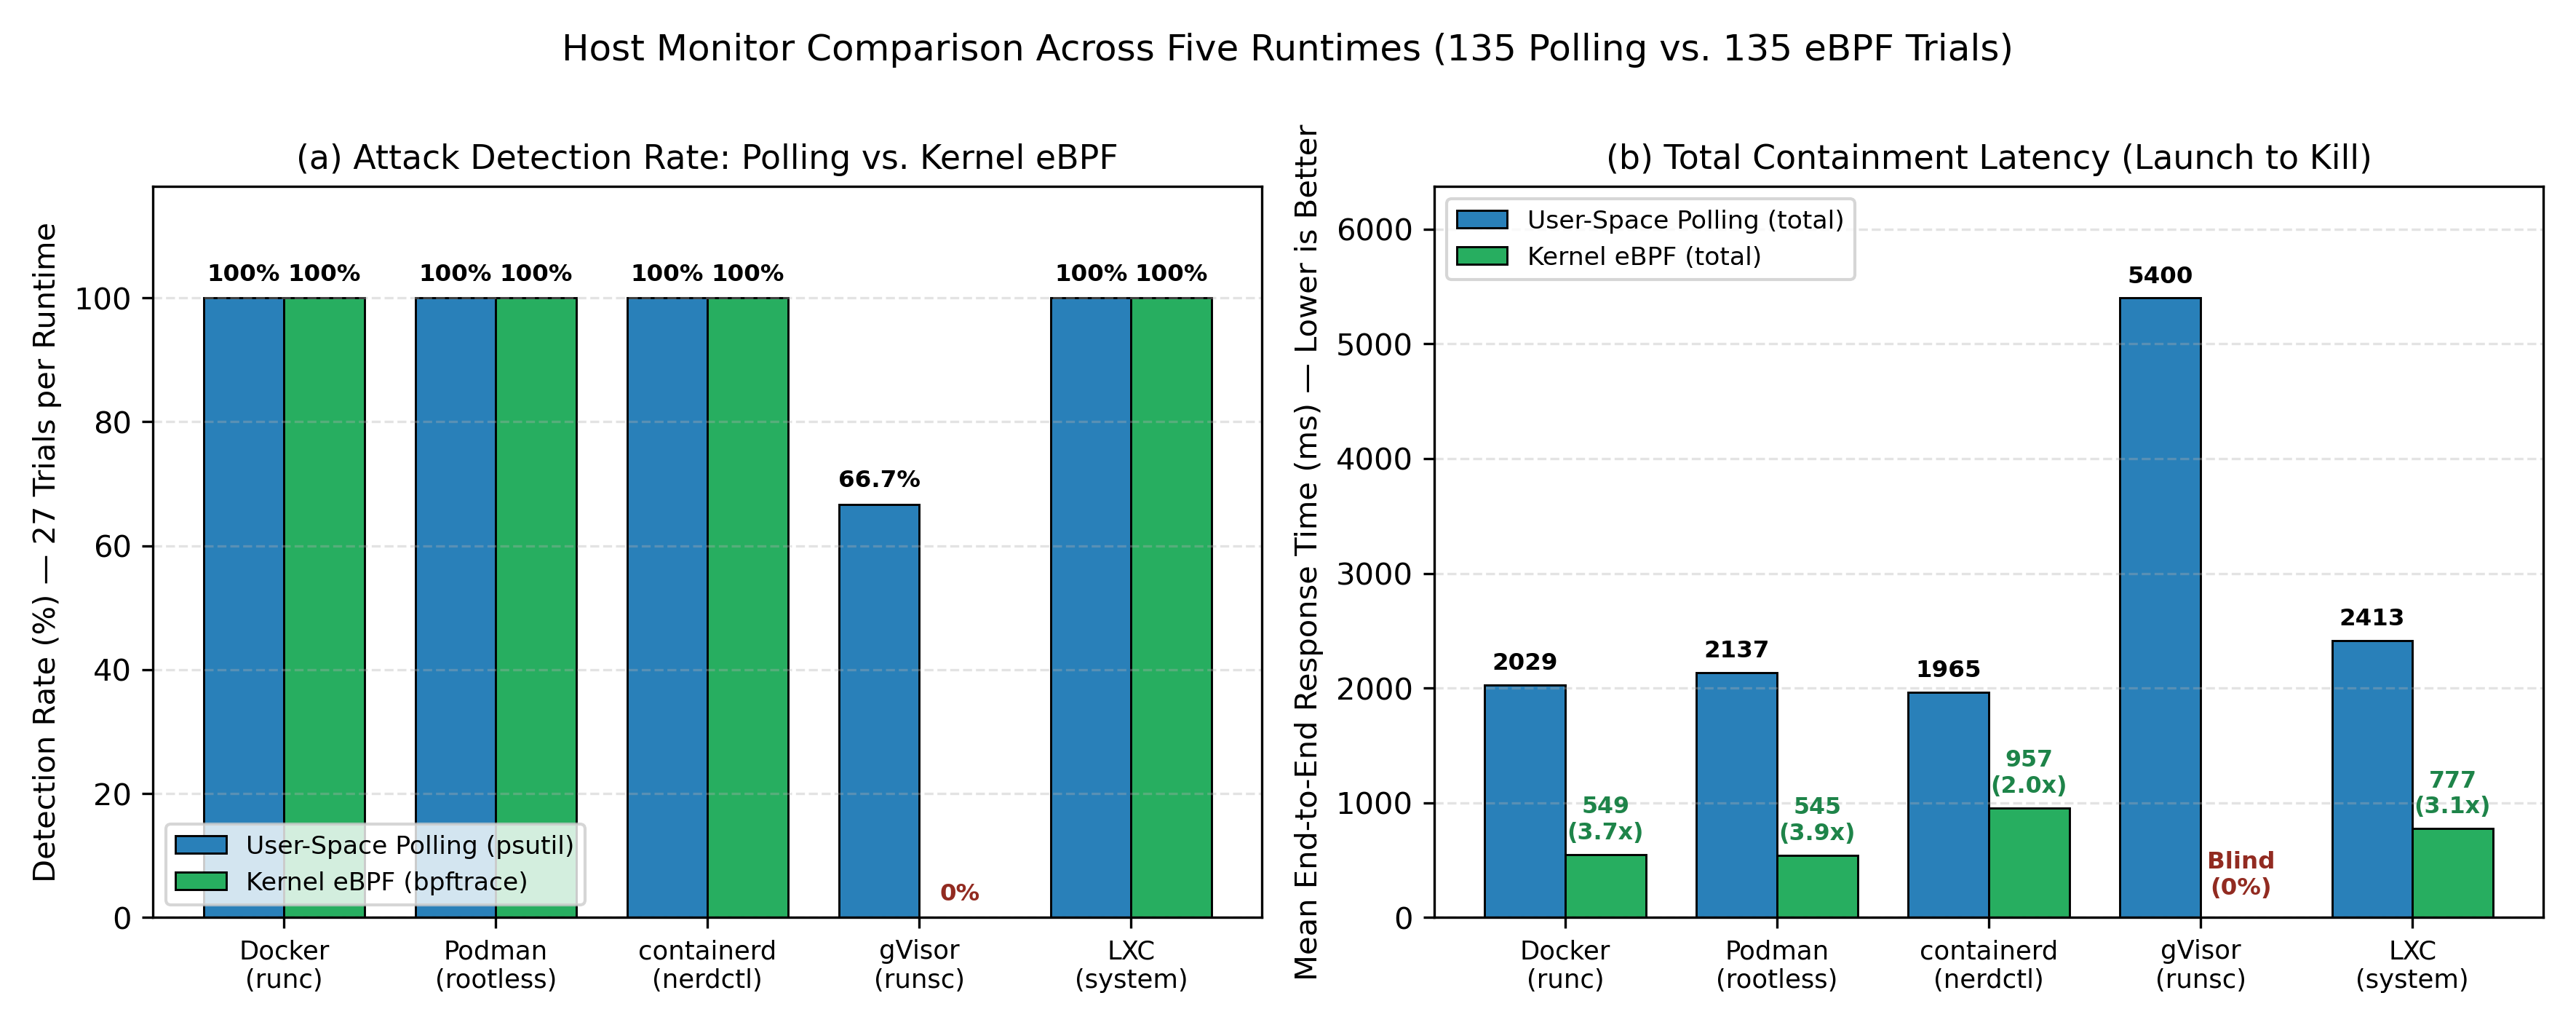
\includegraphics[width=\linewidth]{fig9_ebpf_vs_polling.png}
\caption{User-space polling vs.\ kernel eBPF detection rates and total response times across all five runtimes (270 total trials).}
\label{fig:fig9}
\end{figure}

\begin{figure}[t]
\centering
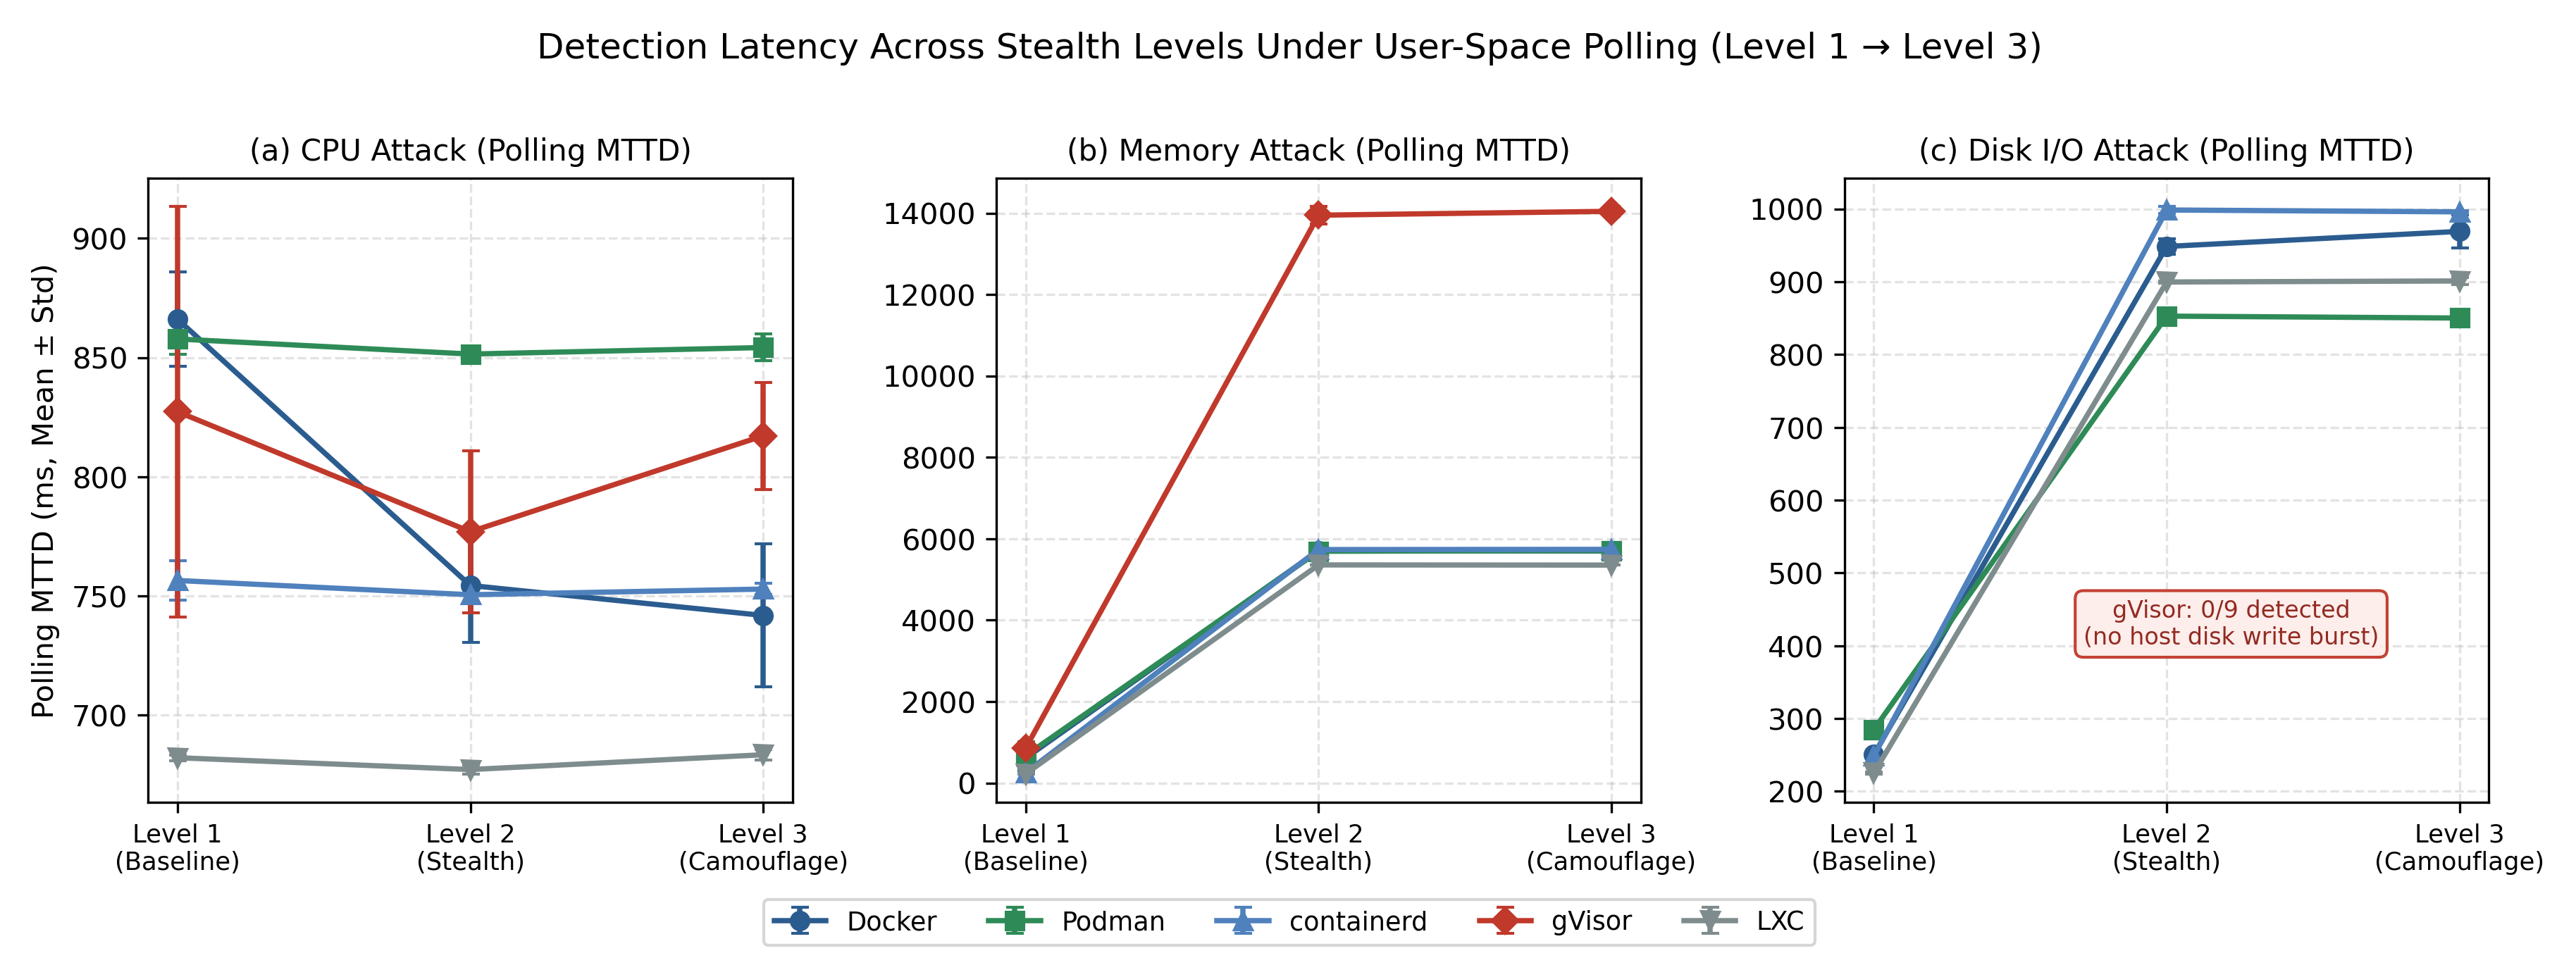
\includegraphics[width=\linewidth]{fig10_gen_evasion_curves.png}
\caption{Polling detection time across stealth Levels~1--3 for all three test attack programs.}
\label{fig:fig10}
\end{figure}

\begin{figure}[t]
\centering
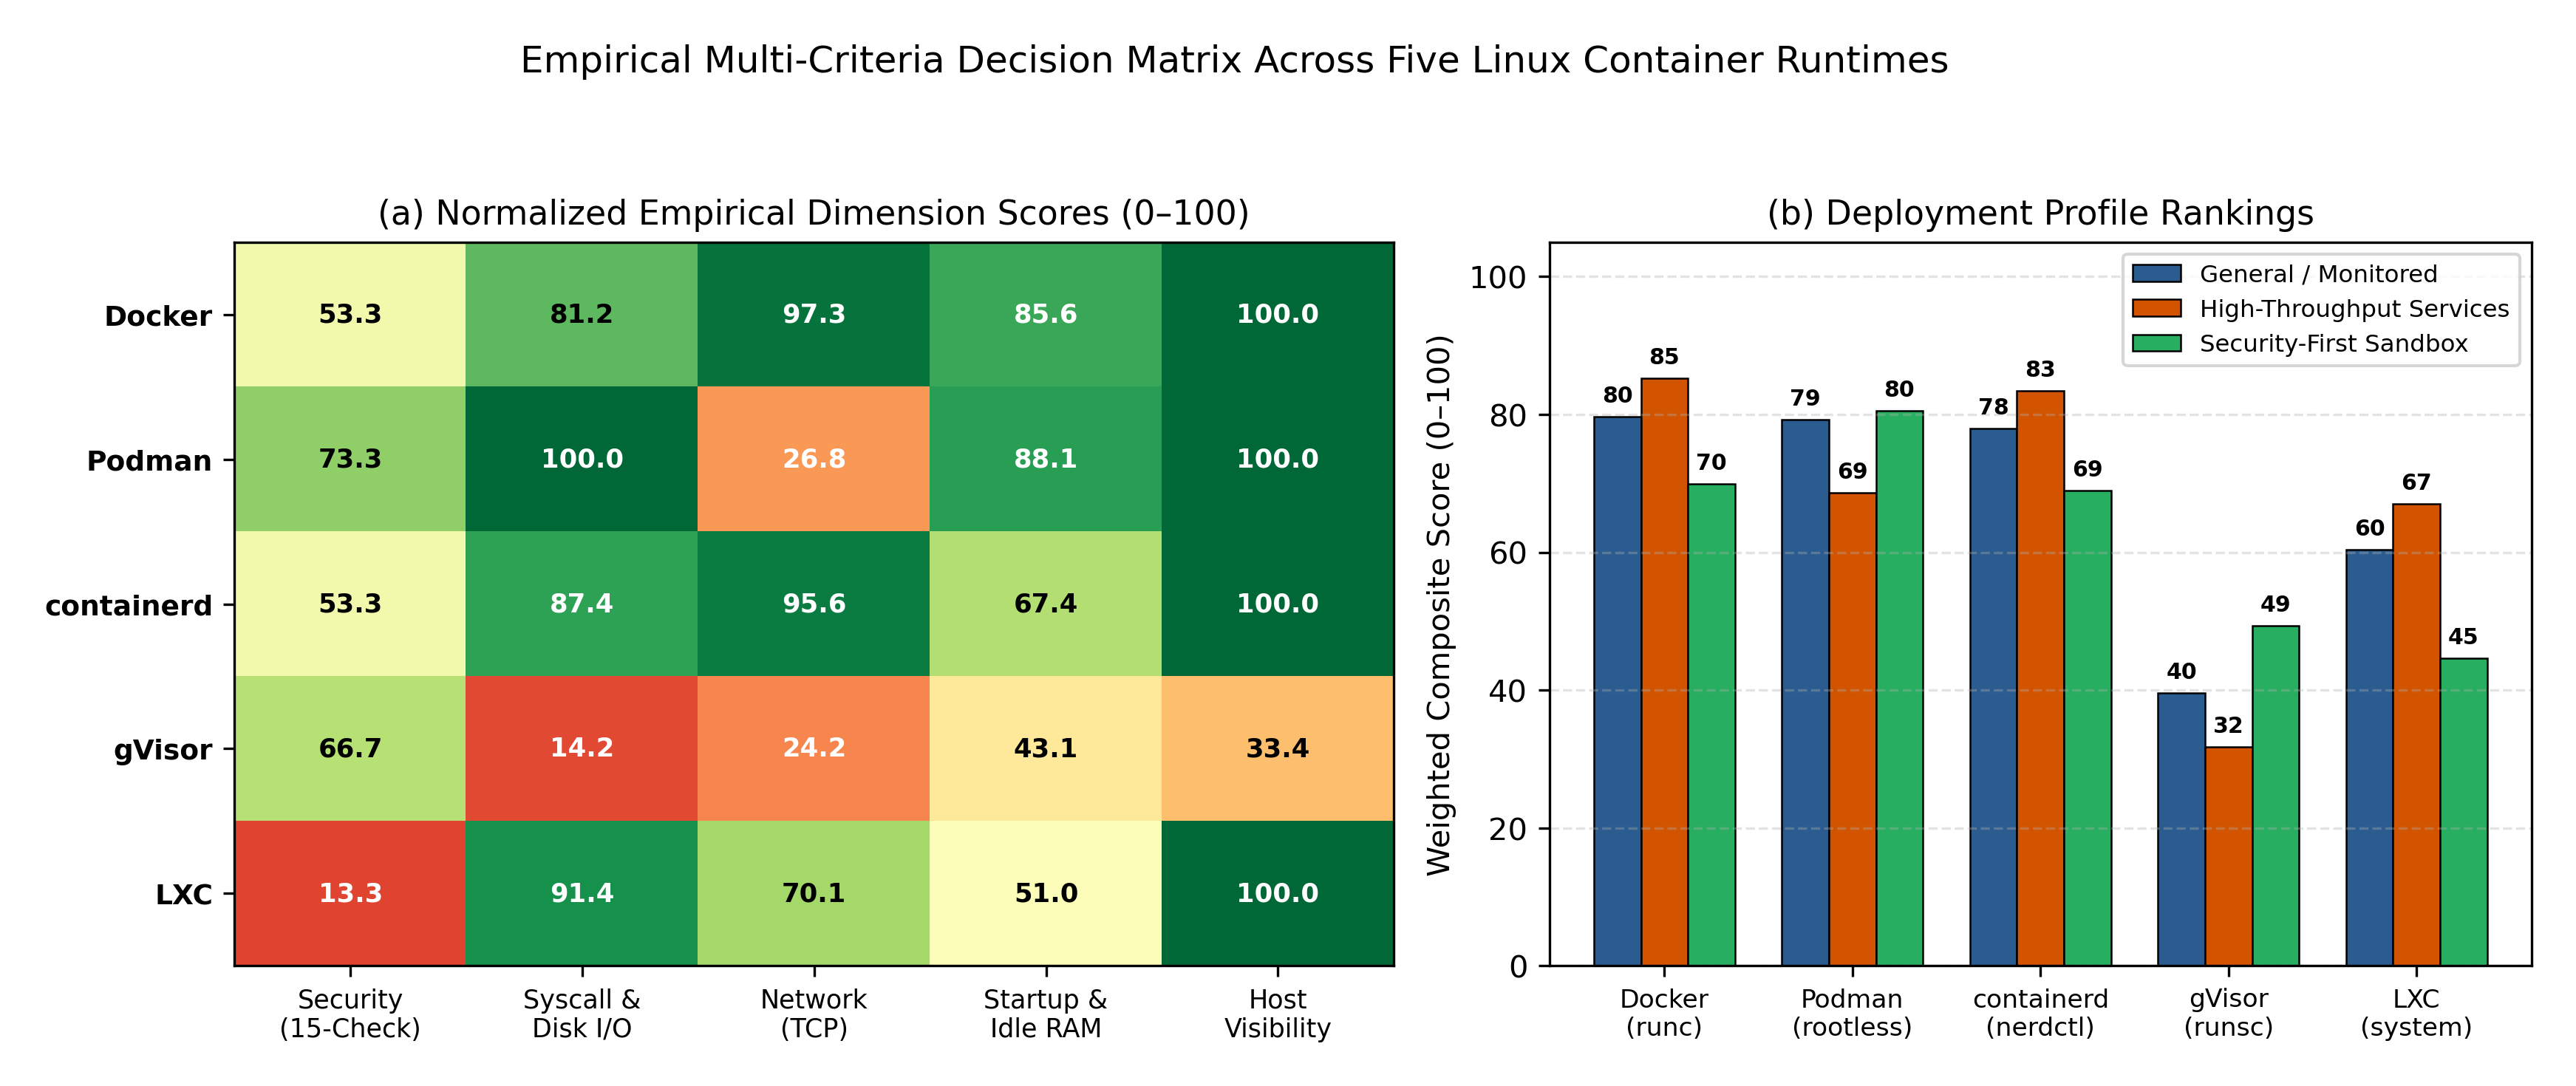
\includegraphics[width=\linewidth]{fig11_weighted_decision_matrix.png}
\caption{Normalized 0--100 dimension scores and weighted rankings across three example use cases.}
\label{fig:fig11}
\end{figure}

\section{Discussion}

\textbf{Why Performance Differed:} Our Module~2 results explain the disk I/O gap from Module~1 and align with prior work on gVisor~\cite{young2019}. Shared-kernel runtimes pass system calls directly to the host Linux kernel, keeping latency close to bare metal. gVisor intercepts system calls inside its user-space Sentry layer~\cite{gvisor}, which creates heavy overhead on syscall-intensive and memory-mapping workloads. Networking revealed a separate trade-off: routing traffic through user-space networking in Podman and gVisor blocked raw ICMP sockets, but substantially slowed down container-to-host TCP latency and throughput compared to Docker, containerd, and LXC.

\textbf{Two Different Approaches to Security:} Rootless Podman and gVisor protect the host in different ways. gVisor shields the host kernel itself by running Sentry in between. However, because we ran gVisor through rootful Docker, container root could still read a bind-mounted host root secret file. Rootless Podman prevented that read through UID remapping, showing how effective unprivileged user namespaces are against file-sharing mistakes. Meanwhile, Docker and containerd produced identical security results because both use the same default \texttt{runc} rules, and default rootful LXC left the widest attack surface open~\cite{lin2018}.

\textbf{Cgroups v2 Are Mandatory on Every Runtime:} Choosing a more isolated runtime does not automatically protect a server from resource-exhaustion attacks. Under default settings, all five runtimes allowed the full 500-process fork bomb and let an 8-thread CPU workload cut host speed nearly in half. Setting explicit cgroup v2 process and CPU caps solved both problems across every runtime.

\textbf{The Isolation vs.\ Visibility Trade-Off:} Strong kernel separation comes with a monitoring blind spot. While kernel eBPF detected every attack in milliseconds and stopped stealth evasion on Docker, Podman, containerd, and LXC, the exact Sentry boundary that protects the host kernel in gVisor also blinded our host eBPF monitor completely. Teams running gVisor therefore cannot rely only on standard host-kernel eBPF sensors.

\textbf{Limitations:} All tests ran inside a single 4-vCPU virtual machine to keep hardware identical across runtimes; absolute speeds on bare-metal servers may differ. In addition, Module~1 ran on kernel \texttt{7.0.0-38-generic} while Modules~3 and~4 ran on \texttt{7.0.0-43-generic} after a routine Ubuntu update, and we evaluated default runtime settings rather than custom-hardened security profiles or unprivileged LXC.

\section{Conclusion and Recommendations}
No single container runtime won every category across our four modules. The best choice depends on what a system prioritizes:
\begin{itemize}
    \item \textbf{Security-First and Balanced General Use --- Rootless Podman:} Earned the top security-first score in Table~\ref{tab:m4_matrix}, blocked host root bind-mount reads, matched native syscall and disk speeds, and kept 100\% host monitoring visibility, provided slower container-to-host TCP networking is acceptable.
    \item \textbf{Network-Heavy and High-Throughput Services --- Docker and containerd:} Delivered the fastest TCP speeds, near-native syscalls, and full eBPF monitoring visibility, making Docker the top scorer for both high-throughput and general monitored setups. Operators should still drop unneeded capabilities (like \texttt{CAP\_NET\_RAW}) and set cgroup limits.
    \item \textbf{Untrusted Code Requiring Kernel Protection --- gVisor:} Although syscall, disk, network, and host eBPF limitations lowered its composite scores, gVisor is the only runtime tested that separates untrusted code from the host Linux kernel with a user-space kernel.
    \item \textbf{Legacy Full-OS Workloads Only --- LXC:} Offers fast startup and native compute speed, but default rootful LXC leaves too many dangerous capabilities open to host untrusted code safely without unprivileged configuration.
\end{itemize}

Future work can test custom hardened configurations (such as dropping all capabilities and running unprivileged LXC) and compare gVisor against lightweight microVM runtimes such as Firecracker or Kata Containers.

\begin{thebibliography}{7}
\bibitem{felter2015} W. Felter, A. Ferreira, R. Rajamony, and J. Rubio, ``An Updated Performance Comparison of Virtual Machines and Linux Containers,'' in \textit{Proc. IEEE Int. Symp. Performance Analysis of Systems and Software (ISPASS)}, 2015, pp. 171--172.
\bibitem{young2019} E. G. Young, P. Zhu, T. Caraza-Harter, A. C. Arpaci-Dusseau, and R. H. Arpaci-Dusseau, ``The True Cost of Containing: A gVisor Case Study,'' in \textit{Proc. 11th USENIX Workshop on Hot Topics in Cloud Computing (HotCloud '19)}, 2019.
\bibitem{lin2018} X. Lin, L. Lei, Y. Wang, J. Jing, K. Sun, and Q. Zhou, ``A Measurement Study on Linux Container Security: Attacks and Countermeasures,'' in \textit{Proc. 34th Annual Computer Security Applications Conference (ACSAC '18)}, 2018, pp. 418--429.
\bibitem{sultan2019} S. Sultan, I. Ahmad, and T. Dimitriou, ``Container Security: Issues, Challenges, and the Road Ahead,'' \textit{IEEE Access}, vol. 7, pp. 52976--52996, 2019.
\bibitem{gregg2019} B. Gregg, \textit{BPF Performance Tools: Linux System and Application Observability}. Boston, MA, USA: Addison-Wesley Professional, 2019.
\bibitem{gvisor} Google, ``gVisor: Application Kernel for Containers,'' \url{https://gvisor.dev/docs/}, accessed Nov. 2026.
\bibitem{podman} Red Hat, ``Podman: Daemonless, Rootless Linux Containers,'' \url{https://podman.io/}, accessed Nov. 2026.
\end{thebibliography}

\end{document}
